\documentclass[german, version-2020-11]{uzl-thesis}

\UzLThesisSetup{
    Logo-Dateiname          = {res/imis-thesis-logo.pdf},
    Verfasst                = {am}{Institut für Multimediale und Interaktive Systeme},
    Titel auf Deutsch       = {
        AR-Event-App Framework für ortsbezogene Veranstaltungen
    },
    Titel auf Englisch 	    = {
        AR-Event-App Framework for location-based Events
    },
    Autor                   = {Raimund Canzler},
    Betreuerin              = {Univ.-Prof. Dr.-Ing. Nicole Jochems Dipl.-Inform.},
    Mit Unterstützung von   = {Torben Volkmann, M.Sc.},
    Bachelorarbeit,
    Studiengang       	    = {Medieninformatik},
    Datum                   = {1. Januar 2022},
    Abstract                = {

    },
    Zusammenfassung         = {

    },
    Alphabetische Bibliographie,
}

\UzLStyle{alegrya modern design}

\addbibresource{sources.bib}


%%%%%%%%%%%%
% GRAFIKEN %
%%%%%%%%%%%%

\graphicspath{ {./res/images/} }

\newcommand{\textgraphics}[2][height=.5cm]{$\vcenter{\hbox{\includegraphics[#1]{#2}}}$}


%%%%%%%%%%%%%%%%
% ANFORDERUNGEN %
%%%%%%%%%%%%%%%%

\usepackage{array}
\usepackage{etoolbox}
\usepackage{longtable}

\newcommand\anfletter{Q}

\newcommand\setanf[1]{\renewcommand\anfletter{#1}}

\newcounter{anfnumber}
\newcounter{anfsubnumber}
\newcommand\showanfnumber{
    \textbf{/\anfletter\arabic{anfnumber}\arabic{anfsubnumber}/}
    \def\@currentlabel{/\arabic{anfnumber}\arabic{anfsubnumber}/}
    \label{anf:\anfletter\arabic{anfnumber}\arabic{anfsubnumber}}
}

\newcommand\anfrow{\setcounter{anfsubnumber}{0}\refstepcounter{anfnumber}\showanfnumber}
\newcommand\anfsubrow{\refstepcounter{anfsubnumber}\showanfnumber}

\newcommand{\anfref}[1]{\hyperref[anf:#1]{/#1/}}

\preto\tabular{\setcounter{anfnumber}{0}}
\preto\tabular{\setcounter{anfsubnumber}{0}}

\preto\longtable{\setcounter{anfnumber}{0}}
\preto\longtable{\setcounter{anfsubnumber}{0}}



%%%%%%%%%%%%
% DOKUMENT %
%%%%%%%%%%%%

\begin{document}

\setlength{\parindent}{0em}
\setlength{\parskip}{1em}

\chapter{Einleitung}

% TODO: Quellen überprüfen!

In den letzten 20 Jahren hat sich am Kern der Veranstaltungsorganisation wenig
verändert, jedoch bietet moderne Technik Veranstaltungen eine größere Bühne als
je zuvor. Digitale Medien haben in den letzten 10 Jahren den Zugang zu
Veranstaltungen enorm erleichtert \cite{Bladen2012}. Webinars,
Online-Konferenzen, -Training und -Workshops bieten Menschen quer über die Welt
verteilt die Möglichkeit, an Veranstaltungen teilzunehmen und dabei zu wählen,
was sie wann und wie sehen möchten. Jedoch fehlt reinen Online Veranstaltungen
ein wichtiger Aspekt von örtlich stattfindenden Veranstaltungen: die
Face-to-face Interaktion \cite{Bladen2012}. Soziale Interaktion ist ein wichtiges
psychologisches Grundbedürfnis \cite{Maslow1943}.

Anfang 2021 waren soziale Interaktionen durch die pandemische Lage nur sehr
eingeschränkt möglich. Zum EMI-Award 2021 wurde deshalb am Institut für
Multimediale und Interaktive Systeme (IMIS) der Universität zu Lübeck im Rahmen
eines Bachelor-Projekts die EMI-Award-App umgesetzt \cite{Canzler2021}. Beim
EMI-Award handelt es sich um eine jährliche Veranstaltung des Studiengangs
Medieninformatik, bei welcher „die kreativsten und gelungensten
Gruppenergebnisse aus der Erstsemester-Veranstaltung ‚Einführung in die
Medieninformatik‘ (EMI) ausgezeichnet [werden]“ \cite{UniversitatzuLubeck2021}.
Aufgrund der Kontaktbeschränkung konnten, im Gegensatz zu den vorherigen Jahren,
die Projekte der Studenten nicht im Foyer des Audimax an der Universität zu
Lübeck vorgestellt werden. Die App ermöglicht das Ansehen und Bewerten der im
gesamten Raum Lübeck verteilten Projekte. Innerhalb von 2 Wochen wurde die
Web-App von über 300 Personen genutzt. Teilnehmende erhielten die Möglichkeit,
die Projekte in ihrer eigenen Geschwindigkeit zu erkunden. Zudem ging aus
informellen Erfahrungsberichten hervor, dass Teilnehmende an Projektstandorten
öfter aufeinandertrafen.

% App, welche Veranstaltungen digital unterstüzt
%   - Nutzer einen roten Pfaden bieten
%       - Einführende Informationen zur Veranstaltung
%       - Informieren zu Standorten, Neuigkeiten
%       - Fortschrittsüberblick durch virtuelle Besuche / Einchecken
%       - Gruppen-Funktion
%       - soziale Interaktion durch Reaktionen
%       - Beteiligung durch Gamification
%       - Hilfe anbieten, häufige Probleme lösen
%   - Veranstalter die Informationsverteilung und -aufnahme stark vereinfachen
%       - Überblicken der Veranstaltung
%       - Spontan Feedback sammeln
%       - Jederzeitiges Eingreifen durch Benachrichtigungen
%       - Häufige Probleme dank FAQ abfangen
%       - Datensammlung für Evaluationszwecke
%   - Einfache Nutzung dank Web-App
%   - Keine Registration

\section{Ziele dieser Arbeit} \label{sec:goals}

Im Rahmen dieser Bachelorarbeit wurde eine Erweiterung und Verallgemeinerung der
EMI-Award-App in Form eines flexiblen Event-App-Frameworks für ortsbasierte
Veranstaltungen konzipiert und entwickelt. Dabei wurde die Organisation von
Veranstaltungen und Teilnahme näher analysiert. Zudem wurden die Vor- und
Nachteile der bestehenden Anwendung einbezogen. Das Framework unterstützt
Veranstaltende ab der „Umsetzung“ und Teilnehmende ab der „Durchführung“ einer Veranstaltung.

Veranstaltende können über ein Online-Dashboard ihre Veranstaltung verwalten.
Dies umfasst das Anlegen von verschiedenen Standorten, Abzeichen und
Hilfseinträge. Des Weiteren sollen Push-Nachrichten sowie Feedbackanfragen an
alle Teilnehmenden abgeschickt werden können. Zusätzlich ermöglicht die Web-App
Daten zu besuchten Standorten, erhaltenen Abzeichen und Feedback gesammelt
darzustellen. Diese Daten können anschließend zur Auswertung der Veranstaltung
genutzt werden.

Teilnehmenden wird durch die Darstellung wichtiger Informationen
zur Veranstaltung ein roter Faden geboten. Dies geschieht mithilfe einer
Anzeige der Standorte, sowohl auf einer interaktiven Karte, als auch in
Listenform. Zudem können weitere Informationen und multimediale Inhalte zu den
einzelnen Standorten eingesehen werden. Durch die Realisierung von virtuellen Besuchen an bestimmten Standorten per QR-Code und die Möglichkeit des Sammelns von Abzeichen können Teilnehmende dazu angeregt werden, bestimmte Aktionen auszuführen.

\section{Aufbau der Arbeit}

Die Entwicklung des Frameworks orientiert sich am menschenzentrierten
Gestaltungsprozess \citedin{DINISO9241}. Der Prozess teilt im Rahmen dieser
Arbeit in vier aufeinanderfolgende Phasen (\autoref{fig:vorgehen}).

\begin{figure}[htpb]
    \centering
    
\includegraphics[width=\linewidth]{vorgehen.png}
    \caption{Das Vorgehen dieser Bachelorarbeit}
    \label{fig:vorgehen}
\end{figure}

In der ersten Phase (s. \autoref{chapter:analysis}) wurden die Anforderungen an das zu erstellende Framework
erarbeitet. Zuerst wurde Nutzungskontext des Frameworks analysiert. Hierzu
wurden eine Literaturrecherche und Interviews mit Teilnehmenden und
Veranstaltenden durchgeführt, um ein besseres Verständnis für die Planung und
Durchführung von Veranstaltungen, sowie der Probleme in diesen Phasen, zu
erlangen. Des Weiteren wurde das bestehende System, die EMI-Award-App,
analysiert, um den Stand der Technik zu beleuchten. Abschließend wurden die
gesammelten Erkenntnisse in Form von formalen Anforderungen festgehalten.

Während der Konzeptionsphase (s. \autoref{chapter:conception}) wurden, auf Basis der formalen Anforderungen,
Funktionalitäten des Frameworks konzipiert. Hierbei wurde auf den
Funktionalitäten des bestehenden Systems aufgebaut und weitere Funktionalitäten
hinzugefügt, um die Anforderungen abzudecken. Anschließend wurde das
Interfacedesign der Frame\-work-Kom\-po\-nen\-ten entwickelt. Abschließend
wurden auf Grundlage der Anforderungen die zu nutzenden Frameworks festgelegt
und darauf aufbauend die Systemarchitektur festgelegt.

Zur Implementierungsphase (s. \autoref{chapter:implementation}) wurden die zuvor konzipierten Entwürfe des Systems
realisiert. Hierbei wurden die in der Konzeptionsphase festgelegten Frameworks
genutzt. Im anschließenden Kapitel wurde das realisierte System anhand von
Dialogbeispielen präsentiert (s. \autoref{chapter:dialog}).

In der letzten Phase (s. \autoref{chapter:evaluation}) wurde das entwickelte System von Teilnehmenden und
Veranstaltenden evaluiert. Für die Seite der Veranstaltenden wurde erhoben,
inwieweit das System in der Organisation und Durchführung unterstützt. Ein
besonderes Merkmal wird hierbei auf die Überwachung der Veranstaltung gesetzt.
Durch die Teilnehmenden wurde erhoben, ob und wie sehr die implementierten
Funktionalitäten zur Orientierung während des Besuchs der Veranstaltung
unterstützen konnten. Abschließend werden die Ergebnisse diskutiert und ein
Ausblick über offene Punkte, mögliche Erweiterungen und Weiterentwicklungen des
Systems gegeben (s. \autoref{chapter:summary}).

% \begin{figure}[htpb]
%     \renewcommand\baselinestretch{1}
%     \centering
%     \tikzset{
%         textbox/.style={
%                 text width=4cm,
%                 text centered,
%                 align=center
%             },
%         arrow/.style={
%                 ->
%             }
%     }
%     \tikz [thesis box shapes, baseline, anchor=base]{
%         \node [block] (1) [textbox] at (-3, 8) {Den menschenzentrierten
%             Gestaltungsprozess planen};
%         \node [block] (2) [textbox] at (0, 3.75) {Den Nutzungskontext verstehen und
%             beschreiben};
%         \node [block] (3) [textbox] at (4.5, 0) {Die Nutzungsanforderungen
%             spezifizieren};
%         \node [block] (4) [textbox] at (0, -3) {Gestaltungslösungen entwickeln,
%             die die Nutzungsanforderungen erfüllen};
%         \node [block] (5) [textbox] at (-4.5, 0.25) {Gestaltungslösungen aus der
%             Benutzerperspektive evaluieren};
%         \node [block] (6) [textbox] at (-6, 4.5) {Gestaltungslösung
%             erfüllt die Nutzungsanforderungen};
%         \draw[arrow] (1.south) to [out=270, in=90] (2.north);
%         \draw[arrow, bend left=45] (2.east) to (3.north);
%         \draw[arrow, bend left=45] (3.south) to (4.east);
%         \draw[arrow, bend left=45] (4.west) to (5.south);
%         \draw[arrow] (5.west) to [out=180, in=270] (6.south);
%         \draw[arrow, dashed, bend left=45] (5.north) to (2.west);
%         \draw[arrow, dashed, bend left=35] (5.north) to (3.north);
%         \draw[arrow, dashed, bend left=75] (5.north) to (4.north);
%         \node [fill=white, fill opacity=0.7, text width=4cm, text opacity=1] (7) at (-3.5, 2) {Iteration, soweit
%             Evaluationsergebnisse Bedarf hierfür aufzeigen};
%     }
%     \caption{Der menschenzentrierte Gestaltungsprozess \citedin{DINISO9241}}
%     \label{fig:din-hcd}
% \end{figure}


\chapter{Analyse}

Um entscheidende Rahmenbedingungen für das Projekt festlegen zu können und
diverse Einflüsse auf die Entwicklung, sowie die spätere Nutzung des Systems
einschätzen zu können, wurde in diesem Kapitel eine ganzheitliche Analyse
durchgeführt. Aufgrund der vielfältigen Veranstaltungstypen wurden die zu
betrachtenden Veranstaltungen eingegrenzt. Anschließend wurde eine
Organisationsanalyse durchgeführt, um die verschiedenen Phasen einer
Veranstaltung einzubeziehen. Die Phasen „Umsetzung“, „Durchführung“ und
„Schließung“ wurden hierbei näher analysiert. Basierend auf den Ergebnissen der
Organisationsanalyse wurden eine Benutzer- und Kontextanalyse durchgeführt. Die
Zielgruppen des Frameworks wurden festgelegt und für die Konzeption relevante
Besonderheiten herausgearbeitet. In einer abschließenden Kontextanalyse wurden
die verschiedenen Kontexte der Nutzung des Frameworks aufgezeigt und auf die mit
ihnen einhergehenden Herausforderungen eingegangen.


\section{Datenquellen}

Im Rahmen der Analyse wurden verschiedene Datenquellen genutzt. Es wurde eine
wissenschaftliche Literaturrecherche zwischen dem 26.07.2021 und 11.08.2021
durchgeführt. Verschiedene vergleichbare Projekte wurden im Rahmen einer
Internetrecherche ermittelt. Unter anderem wurden die Ausarbeitung und
Evaluation der EMI-Award-App als Quellen genutzt. Zudem wurden Interviews mit
Veranstaltenden und Teilnehmenden durchgeführt, welche zwischen dem 5.09.2021
und 17.09.2021 stattfanden. \\
Zur Literaturrecherche wurden die digitalen Bibliotheken ACM Digital Library
(\url{https://dl.acm.org/}) und Google Scholar
(\url{https://scholar.google.de/}) genutzt. Es wurden Begriffe aus den Bereichen
Event Management (\emph{Event Management, Event Evaluation, Event Experience,
    Event Tracking}) und UX (\emph{Attention Economy, Attention Management,
    Information Overload, Digital Burnout, Overchoice, Web Animation, Animation UX,
    UX Micro Interaction, Animation Usability}) zur Suche verwendet. \\
Die Interviews mit Veranstaltenden und Teilnehmenden wurden qualitativ und
semistrukturiert, mit Hilfe eines dafür entworfenen Interviewleitfadens (siehe
Anhang A), durchgeführt. Bei den Veranstaltenden handelt es sich um Personen mit
praktischer Erfahrung in der Organisation von Veranstaltungen. In Tabelle
\ref{table:ver-soz} und Tabelle \ref{table:teil-soz} sind Details zu den
befragten Personen aufgelistet. Die IDs der interviewten Personen werden im
Verlauf der Analyse referenziert.

\begin{table}[htpb]
    \def\arraystretch{1.25}
    \centering
    \caption{Soziodemografische Daten der Veranstaltenden}
    \label{table:ver-soz}
    \begin{tabular}{lcl}
        \uzlhline
        \uzlemph{ID} & \uzlemph{Alter} &
        \uzlemph{Vorerfahrung}                         \\
        \uzlhline V1 & 40 - 59 J.      & Verschiedene
        Veranstaltungen, verteilt über 11 Jahre        \\
        V2           & 18 - 25 J.      & Mehrere große
        Veranstaltung (>2000 Teilnehmende)             \\
        \uzlhline
    \end{tabular}
\end{table}

\begin{table}[htpb]
    \def\arraystretch{1.25}
    \centering
    \caption{Soziodemografische Daten der Teilnehmenden}
    \label{table:teil-soz}
    \begin{tabular}{lccl}
        \uzlhline
        \uzlemph{ID}                     & \uzlemph{Alter}     &
        \uzlemph{EMI-Award-App genutzt?} & \uzlemph{Tätigkeit}
        \\
        \uzlhline T1                     & 18 - 25 J.          & j
                                         & Student:in              \\
        T2                               & 18 - 25 J.          & j
                                         & Student:in              \\
        T3                               & 18 - 25 J.          & j
                                         & Student:in              \\
        T4                               & 18 - 25 J.          & n
                                         & Student:in              \\
        T5                               & 40 - 59 J.          & n
                                         & Berufstätig             \\
        \uzlhline
    \end{tabular}
\end{table}


\section{Definition: Veranstaltung} \label{sec:analysis-def}

Bevor die verschiedenen Aufgaben, Probleme und Benutzergruppen analysiert werden
können, müssen Umfang und Typ der Veranstaltung festgelegt werden. In der
Literatur sind verschiedene Definitionen zum Begriff „Veranstaltungen“ zu
finden, welche sich in Umfang und Inhalt unterscheiden. Die räumliche und
zeitliche Dimension von Veranstaltungen ist sehr flexibel. \textcite{Getz2007}
definiert Veranstaltungen als zeitliche Phänomene. Bei geplanten Veranstaltungen
wird das Veranstaltungsprogramm oder der Zeitplan im Allgemeinen detailliert
geplant und im Voraus gut bekannt gemacht. Geplante Veranstaltungen sind in der
Regel auch auf bestimmte Orte beschränkt, wobei es sich um eine bestimmte
Einrichtung, eine sehr große Freifläche oder viele Orte handeln kann.
\textcite{Bladen2017} definieren Veranstaltungen als zeitlich begrenzte und
zweckgebundene Zusammenkünfte von Menschen definiert.

Im Rahmen dieser Arbeit werden Veranstaltungen betrachtet, welche in ihrer
zeitlichen Dimension uneingeschränkt sind, jedoch räumlich verteilt stattfinden.
Konkret können die betrachteten Veranstaltungen wenige Stunden, Wochen oder ohne
festgelegtes Ende stattfinden. Zudem verteilen sich die Aktivitäten der
Veranstaltung auf einen größeren Raum. Dies kann mindestens die Aufteilung auf
verschiedene Räumlichkeiten sein, bis hin zur Verteilung über verschiedene
Stadtteile.


\section{Organisationsanalyse} \label{sec:analysis-org}

% Masterarbeit_Holtz  Aufgabenanalyse!!!
Die hier analysierte Vorgehensweise in der Organisation von Veranstaltungen
basiert auf dem EMBOK-Model \cite{Silvers2013} und den Aussagen der interviewten
Veranstaltenden. Typischerweise lässt sich die Organisation von Veranstaltungen
in 5 Phasen (s. \autoref{fig:embok-phases}) gliedern: Initiation, Planung,
Umsetzung, Durchführung und Schließung. Die Vorgehensweise in den Phasen
gestaltet sich wie folgt:

\begin{enumerate}
    \setlength{\itemsep}{1em}
    \item \textbf{Initiation} \\
          Es wird geforscht, um ein Konzept zu erstellen und zu validieren.
          Umfang und Kontext sowie Ziele und Aufgaben werden festgesetzt.
    \item \textbf{Planung} \\
          Anforderungen und Spezifikationen werden festgehalten. Hierzu zählen
          die stattfindenden Aktivitäten, sowie die Art der Organisation und
          erforderliche Ressourcen.
    \item \textbf{Umsetzung} \\
          Alle für die Veranstaltung benötigten Waren und Dienstleistungen
          werden in Auftrag gegeben und koordiniert. Der Fokus liegt unter
          anderem auf der Überwachung und Überprüfung des Umfangs und Zeitplans,
          sowie der Kosten und Qualität.
    \item \textbf{Durchführung} \\
          Die veranstaltungsbezogenen Aktivitäten werden aufgenommen. Ab Beginn
          dieser Phase ist der Handlungsrahmen stark eingeschränkt, wodurch der
          Fokus auf der Überwachung der Veranstaltung liegt.
    \item \textbf{Schließung} \\
          Nach Abschluss der Veranstaltung werden Daten gesammelt, ausgewertet
          und weitergegeben. Das Ziel ist die Dokumentation der Erkenntnisse für
          weitere Veranstaltungen.
\end{enumerate}

\begin{figure}[htpb]
    \centering
    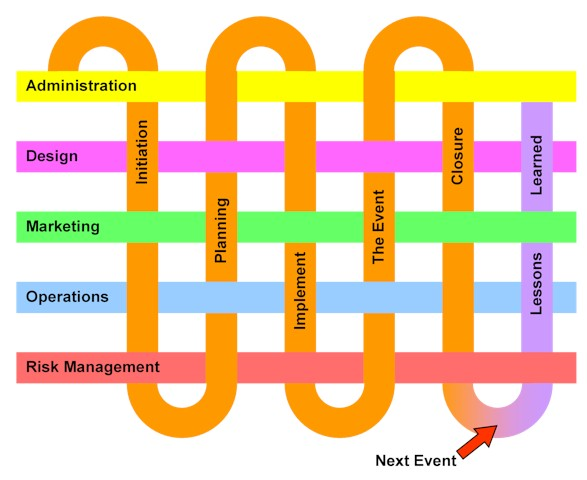
\includegraphics[width=\textwidth]{embok_phases.jpg}
    \caption{Die Phasen der Veranstaltungsorganisation \cite{Silvers2013b}. Die
        verschiedenen Phasen (vertikal) bilden die Grundlage einer
        Veranstaltung. Verwoben sind diese mit Wissensdomänen (horizontal).
        Sollte einer der Fäden verschwinden, wird das gesamte Geflecht
        geschwächt.}
    \label{fig:embok-phases}
\end{figure}

% TODO: Abbildungstext in text einbinden
% TODO: Wissensdomänen erklären

Weil das Ziel dieser Arbeit die Unterstützung ab der Umsetzung ist (s.
\autoref{sec:goals}), werden die Phasen „Umsetzung“, „Durchführung“ und
„Schließung“ näher betrachtet.

\subsection{Umsetzung} \label{sec:analysis-org-umsetzung}

In dieser Phase werden die herausgearbeiteten Pläne umgesetzt. Hierbei werden
Umfang, Zeitpläne, Kosten, Kommunikation und Risiken überwacht und kontrolliert,
um die plangemäße Ausführung sicherzustellen. Weitere Arbeits-/Hilfskräfte
werden engagiert, um bei der Umsetzung mitzuwirken. Für den Erfolg der
Veranstaltung ist die effektive Kommunikation wichtig. Um diese zu
gewährleisten, muss eine Kommunikationsinfrastruktur für Organisierende,
Mitwirkende und externe Dienstleister eingeführt werden. Hilfskräfte müssen in
die Kommunikationsinfrastruktur eingewiesen werden. Aufgrund von mangelnden
technischen Fähigkeiten können bei komplexeren Infrastrukturen Probleme
auftreten (V2).

\subsection{Durchführung} \label{sec:analysis-org-durchfuehrung}

Mit Beginn der Durchführung ändert sich die Dynamik der Veranstaltung bedeutend.
Aufgrund der Anwesenheit von Teilnehmenden sind tiefgreifende Änderungen nun
nicht mehr möglich und beschränken sich auf die Behebung von kleinen Problemen
(V2). Hingegen wird die wichtigste Aufgabe die Überwachung der Veranstaltung.
Unter besonderer Beobachtung stehen logistische Tätigkeiten, sowie unerwartet
auftretende Probleme (V1, V2). Diese können u. a. durch Teilnehmende,
stattfindende Aktivitäten oder die Umgebung der Veranstaltung ausgelöst werden.
\\
Während Probleme, welche die Durchführung der Veranstaltung direkt
beeinträchtigen könnten, streng beobachtet und behoben werden, stehen die
Interaktionen und Erfahrungen der Teilnehmenden zunächst im Hintergrund.
Abgesehen von kritischem Feedback, wird die Erfahrung erst während der
Schließung erfasst und ausgewertet (V2).

\subsection{Schließung} \label{sec:analysis-org-schliessung}

% Bedeutung Evaluation aus Finischen Case S.57-59 Mischung Quantitativ &
% Qualitativ Evaluation S.61

Zur Schließung der Veranstaltung wird die Evaluation zur bedeutendsten Aufgabe.
Feedback und Daten werden von organisierender Seite gesammelt. Hierbei wird
zwischen \textit{weichen} und \textit{harten Daten} unterschieden. Harte Daten
bestehen aus Teilnehmerzahlen, Andrang an verschiedenen Aktivitäten, Dauer,
Einkommen und weiteren zählbaren Merkmalen. Im Vergleich dazu bestehen weiche
Daten u. a. aus Beschwerden, Konflikten, Problemen, Komplimenten, Reaktionen und
Empfehlungen. Mitwirkende, Hilfskräfte und die Organisierenden werden meist dazu
in einer Nachbesprechung befragt (V1,V2). Das Feedback von Teilnehmenden wird
oft nur passiv vor Ort vom Personal erfasst und weitergegeben oder beschränkt
sich auf Familie und Freunde (V2). Die erfassten Erkenntnisse werden
dokumentiert, um auf das Wissen in der nächsten Veranstaltung zurückgreifen zu
können.


\section{Benutzeranalyse} \label{sec:analysis-user}

Um die Funktionen des Frameworks zielgruppengerecht gestalten zu können, werden
in diesem Abschnitt die Benutzergruppen des Frameworks festgelegt und näher
analysiert. Zu den Benutzergruppen gehören Veranstaltende, sowie Teilnehmende
einer Veranstaltung.

\subsection{Veranstaltende}

Inzwischen existieren weltweit tausende Einrichtungen, welche formale
Qualifikationen und Ausbildungen im Veranstaltungsmanagement anbieten. Jedoch
sind diese Qualifikationen nicht einheitlich festgelegt, was zu
unterschiedlichen Schwerpunkten, Umfang, Vermittlungsart und letztendlich
erworbenen Qualifikationen führt \cite{Bladen2017}. In Deutschland gibt es den
anerkannten Ausbildungsberuf des/der Veranstaltungs\-kaufmann/-frau. Die
Aufgaben sind hierbei die Konzipierung und Organisation des kaufmännischen
Aspektes von Veranstaltungen \cite{Kultusministerkonferenz2001}. Die Aufgaben
von Event Manager:innen umfassen zusätzlich die allgemeine Organisation und
Aufgaben im Marketing \cite{BundesagenturfurArbeit2021}. Jedoch ist die
Berufsbezeichnung „Event Manager/in“ rechtlich nicht geschützt. \\
Zudem bedarf es in Deutschland keiner formalen Qualifikation, um eine
Veranstaltung beliebiger Größe zu organisieren. Dementsprechend können keine
bestimmten Qualifikationen für Veranstaltende angenommen werden.
% TODO: Und was bringt das??

\subsection{Teilnehmende}

Die Teilnehmenden einer Veranstaltung unterscheiden sich stark in ihren
soziodemografischen Daten je nach Typ der Veranstaltung. Im Kontext der Arbeit
sind besonders Alter, Technikaffinität und körperliche, seelische, geistige oder
Sinnesbeeinträchtigungen. Für die Betrachtung in dieser Arbeit wird das Alter
der Teilnehmenden auf 16 - 60 J. begrenzt. Zudem wird die sichere grundlegende
Umgangsweise mit einem Smartphone vorausgesetzt.

Da die Literatur zu Event Management ihren Fokus auf die Organisation legt, sind
nur wenig Informationen zur Sicht der Teilnehmenden und ihren Hürden vorhanden.
Als Messwerte für eine erfolgreiche Veranstaltung werden meist
geschäftsrelevante Werte wie z. B. verkaufte Tickets, Teilnehmerzahlen, Umsatz
oder öffentliche Aufmerksamkeit verwendet, welche wenig über die Erfahrung der
Teilnehmenden aussagen. In Interviews wurden die Teilnehmenden gebeten zu
begründen, was eine gewählte Veranstaltung zu ihrem persönlichen Favoriten macht
(s. \autoref{table:teil-fav}).

\begin{table}[htpb]
    \def\arraystretch{1.25}
    \centering
    \caption{Merkmale von positiv empfundenen Veranstaltungen}
    \label{table:teil-fav}
    \begin{tabular}{ll}
        \uzlhline
        \uzlemph{Grund}               & \uzlemph{ID} \\
        \uzlhline  Sozialer Austausch & T1, T2       \\
        Innovative Technik            & T2           \\
        Persönliche Bindung           & T4           \\
        Gute Musik                    & T3           \\
        Einfache Wegfindung           & T5           \\
        Neues Wissen                  & T5           \\
        \uzlhline
    \end{tabular}
\end{table}

\section{Kontextanalyse} \label{sec:analysis-context}

In diesem Abschnitt werden der zeitliche und räumliche Kontext untersucht. Aus
der Beschreibung in \autoref{sec:goals} geht der Fokus auf die Unterstützung von
Veranstaltenden und Teilnehmenden hervor. Die Unterteilung der Benutzergruppen,
wie in \autoref{sec:analysis-user} beschrieben, ist zu beachten. Hieraus ergeben
sich unterschiedliche räumliche und zeitliche Kontexte für Veranstaltende und
Teilnehmende.

Die Unterstützung der Veranstaltenden findet in verschiedene Phasen der
Organisation statt. Der zeitliche Kontext kann mit Blick auf
\autoref{sec:analysis-org} in vor, während und nach einer Veranstaltung
unterteilt werden. Vor der Durchführung einer Veranstaltung ist insbesondere die
Vorbereitung von Aktivitäten und Absicherung von Dienstleistungen oder Waren
wichtig. Während der Veranstaltung hingegen findet ein starker Fokuswechsel auf
die Beobachtung und schnelle Behebung von Problemen statt. Nach einer
Veranstaltung sind die Datensammlung und Auswertung, sowie der Wissenstransfer
von Bedeutung. \\
Auch beschränken sich die betrachteten Veranstaltungen während der Durchführung
auf den in \autoref{sec:analysis-def} beschriebenen örtlichen Bereich, woraus
sich ein weites gehend unbeschränkter räumlicher Kontext ergibt. Vor und nach
der Veranstaltung werden komplexe Informationen eingetragen oder ausgewertet. Da
die Bildschirmgröße einen großen Einfluss auf die effiziente Verarbeitung von
Informationen hat, wird hierfür von einem Arbeitsplatzsystem ausgegangen. Somit
ergibt sich ein räumlich eingeschränkter Kontext vor und nach der Veranstaltung.
Folglich wird während der Veranstaltung ein mobiles System zur Überwachung
benötigt, wobei die Bedingungen vor und nach der Veranstaltung ein stationäres
System befürworten.

Für Teilnehmende ist der Kontext ebenfalls in vor, während und nach der
Veranstaltung aufgeteilt. Der zeitliche Kontext während der Veranstaltung ist
hierbei am bedeutendsten. Auch für Teilnehmende gilt der in
\autoref{sec:analysis-def} beschriebene örtliche Bereich, woraus sich ebenfalls
ein unbeschränkter räumlicher Kontext ergibt. Folglich muss das System für die
Teilnehmenden mobil einsetzbar sein.


\section{Analyse des bestehenden Systems}

An dieser Stelle wird die Implementation und Evaluation der
\textit{EMI-Award-App} vorgestellt, welche die Grundlage des neuen Systems bildet.

% Tech-Stack
%   - Hat sich größten teils bewährt
%   - Web-App mit PWA Funktionalität

% Mockups
%   - Bereits getestet
%   - Grobe Struktur beibehalten

Die \textit{EMI-Award-App} ermöglichte das augmentierte Besuchen, Einsehen und
Bewerten der EMI-Award-Projekte und bildet die Grundlage dieser Arbeit (s.
\autoref{sec:goals}). Speziell wurden dafür an verschiedenen Standorten Schilder
mit QR-Codes angebracht, welche mit einem QR-Code-Reader oder der App gescannt
werden konnten (s. \autoref{fig:emi-qr-code}).

\begin{figure}[htpb]
    \centering
    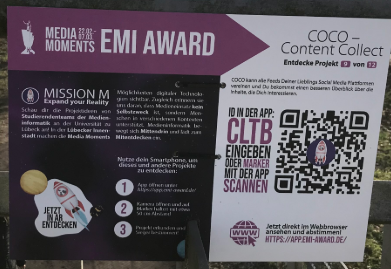
\includegraphics{emi_schild.png}
    \caption{Schild eines Projektstandortes mit QR-Code}
    \label{fig:emi-qr-code}
\end{figure}

Beim ersten Aufruf der App wird dem Nutzenden eine kleine Einführung in die App
und ihren Hintergrund gegeben. Dies geschieht über eine interaktive Slideshow.
Nach dem Bestätigen der letzten Slide werden Nutzende zur interaktiven Karte
geführt (s. \autoref{fig:emi-intro-map}). Auf dieser werden die Projektstandorte
durch verschiedenfarbige Icons von Planeten (\textgraphics{emi_planet.png})
dargestellt. Durch das Antippen eines Standorts wurde eine Kurzinformation, in
Form eines Pop-ups, zum jeweiligen Projekt angezeigt. Außerdem wurde der
Standort des Nutzenden angezeigt, insofern die Berechtigungen dazu gegeben
wurden.

\begin{figure}[htpb]
    \begin{minipage}{.5\textwidth}
        \centering
        
\includegraphics[width=.6\linewidth]{emi_prolog.png}
    \end{minipage}%
    \begin{minipage}{.5\textwidth}
        \centering
        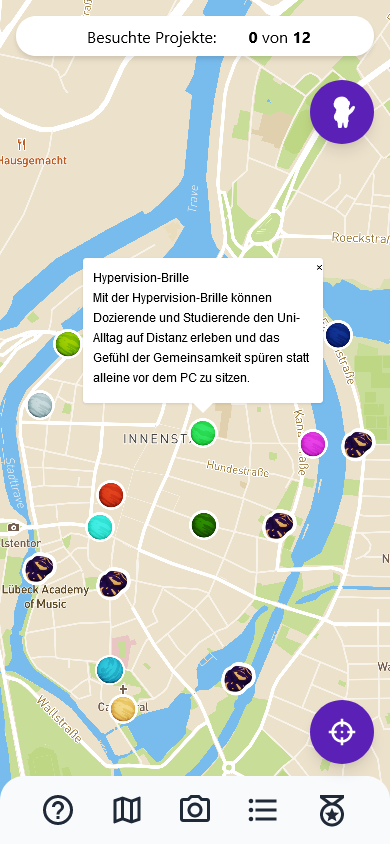
\includegraphics[width=.6\linewidth]{emi_map.png}
    \end{minipage}
    \caption{Einführung und interaktive Karte mit Projektstandorten}
    \label{fig:emi-intro-map}
\end{figure}

Um die vollständigen Informationen eines Projekts einzusehen, musste der
Standort erst virtuell besucht werden. Dies geschah über das Scannen des
QR-Codes auf dem Schild des Standorts (s. \autoref{fig:emi-qr-code}) oder der
manuellen Eingabe eines spezifischen Codes. Nach erfolgreichem Scannen oder
Eingeben des Codes wurde eine virtuelle Szene angezeigt. In dieser musste ein
Planet gesucht und angetippt werden, um den Vorgang abzuschließen (s.
\autoref{fig:emi-ar}). Je nach benutztem Gerät wurde die Szene per Augmented
Reality (AR) oder Virtual Reality angezeigt (VR). Zudem wurde die Anzahl der
besuchten Standorte in der Karten- und Projektansicht anhand eines
Fortschrittsbalkens angezeigt. Die vollständigen Informationen der Projekte
enthielten mediale Inhalte, eine detaillierte Beschreibung und die Autoren des
Projekts. Zusätzlich konnte das Projekt mit einer vorgegebenen Auswahl bewertet
werden (s. \autoref{fig:emi-project}).

\begin{figure}[htpb]
    \begin{minipage}{.5\textwidth}
        \centering
        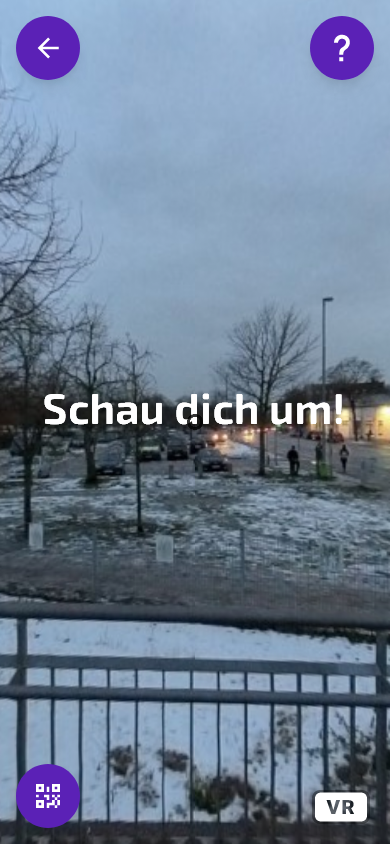
\includegraphics[width=.6\linewidth]{emi_ar-1.png}
    \end{minipage}%
    \begin{minipage}{.5\textwidth}
        \centering
        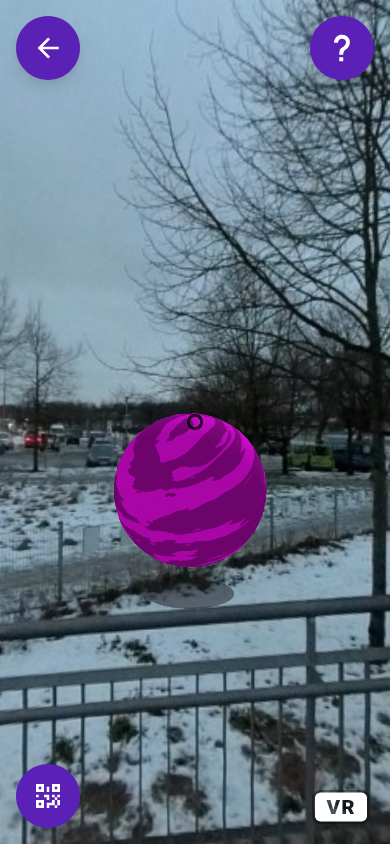
\includegraphics[width=.6\linewidth]{emi_ar-2.png}
    \end{minipage}
    \caption{AR/VR Szene während des virtuellen Besuchs}
    \label{fig:emi-ar}
\end{figure}

\begin{figure}[htpb]
    \begin{minipage}{.5\textwidth}
        \centering
        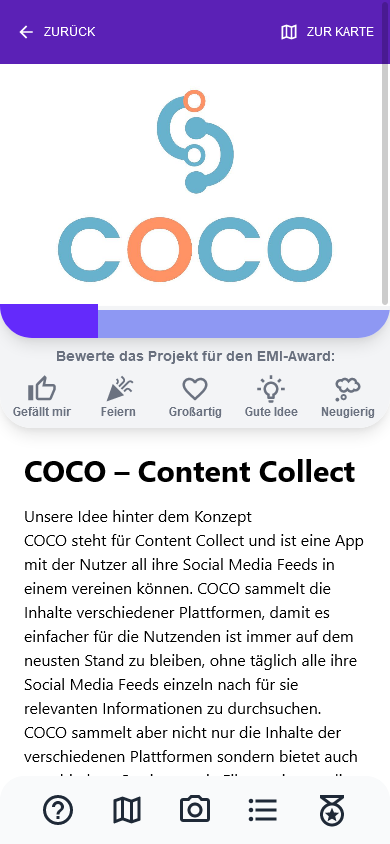
\includegraphics[width=.6\linewidth]{emi_project-1.png}
    \end{minipage}%
    \begin{minipage}{.5\textwidth}
        \centering
        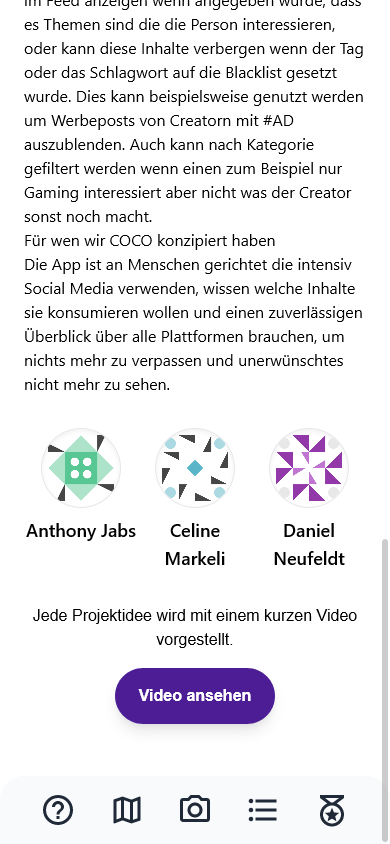
\includegraphics[width=.6\linewidth]{emi_project-2.png}
    \end{minipage}
    \caption{Einzelansicht eines Projekts}
    \label{fig:emi-project}
\end{figure}

Des Weiteren konnten verschiedene Abzeichen für bestimmte Aktionen erhalten
werden. Aktionen waren z. B. das Besuchen einer bestimmten Anzahl von Projekten
oder Benutzen von bestimmten Funktionen. Alle Abzeichen und ihr Fortschritt
konnten in einer Übersicht eingesehen werden (s. \autoref{fig:emi-achievments}).
Bestimmte Abzeichen wurden in mehreren Stufen freigeschaltet oder blieben bis
zum Erhalt verborgen. \\
Zudem wurden die gesammelten „Awardteile“ angezeigt. Awardteile sind sammelbare
Objekte, welche auf der Karte mit einem Meteorit-Symbol
(\textgraphics{emi_meteorit.png}) gekennzeichnet waren. Beim Annähern an die
gezeigten Standorte wurde eine Schaltfläche hervorgehoben, welche durch Antippen
das entsprechende Awardteil sammelt.

\begin{figure}[htpb]
    \centering
    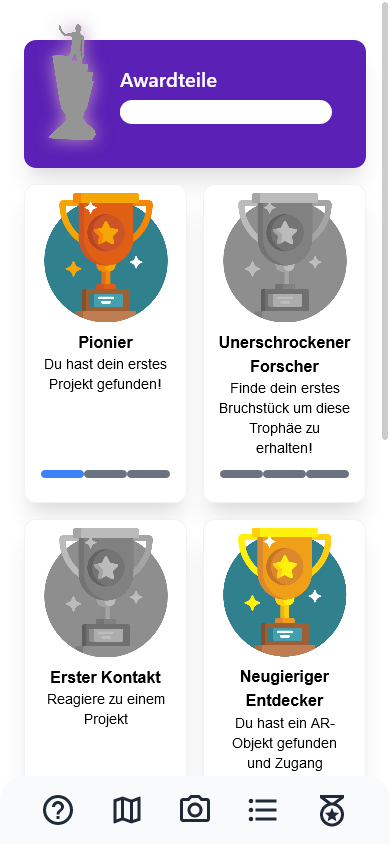
\includegraphics[width=.3\textwidth]{emi_achievements.png}
    \caption{Abzeichen- und Awardteilansicht}
    \label{fig:emi-achievments}
\end{figure}

Außerdem werden die genannten Funktionen in der App durch eine Slideshow
erklärt, welche jederzeit über die Navigationsleiste erreichbar ist (s.
\autoref{fig:emi-help}).

\begin{figure}[htpb]
    \centering
    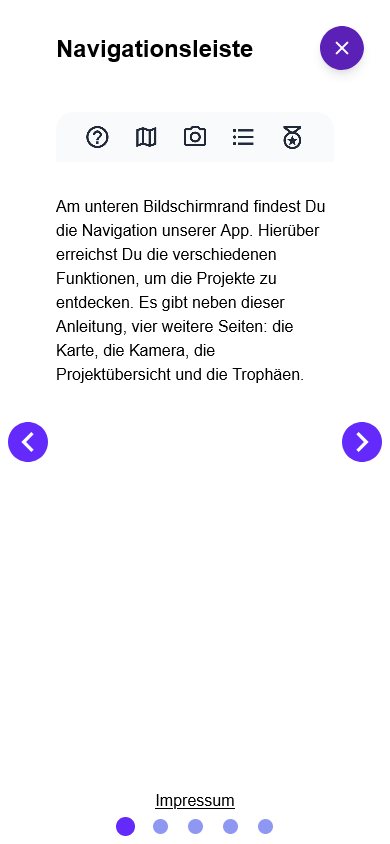
\includegraphics[width=.3\textwidth]{emi_help.png}
    \caption{Eine Seite der In-App-Anleitung}
    \label{fig:emi-help}
\end{figure}

Die EMI-Award-App wurde als progressive Web-App (PWA) realisiert und war unter
\url{https://app.emi-award.de} verfügbar.

Durch die bekannte Evaluation werden die sich etablierten Funktionen in dem
neuen System wiederfinden, außerdem werden die bereits analysierten Punkte in
der Problemanalyse, sowie in den funktionellen Anforderungen mit kombiniert.


\section{Problemanalyse} \label{sec:analysis-problems}

Während Planung, Durchführung und Nachbereitung von Veranstaltungen können
Probleme auftreten, welche die Organisation erschweren. Ähnlich treten bei der
Teilnahme Probleme auf, welche die Erfahrung beeinträchtigen können.

\subsection{Organisation} \label{sec:analysis-problems-orga}

In der Organisation von Veranstaltungen treten vor allem Probleme in der
Kommunikation auf. Je nach Größe der Veranstaltung können eine Vielzahl an
Menschen an der Organisation beteiligt sein. Meist sind verschiedene digitale
Tools oder Plattformen zur Kommunikation erforderlich, um sich mit allen
Veranstaltenden zu verständigen (V2). Hier kann es zu Herausforderungen kommen,
auch Menschen mit geringem Technikverständnis einzuweisen (V2). Aber auch der
Kontakt zu Teilnehmenden spielt eine große Rolle. Jedoch ist der Kontakt während
einer Veranstaltung nur gering (V1, V2). Nach einer Veranstaltung fällt der
Kontakt ebenfalls sehr schwer (V1) oder wird ausgelassen (V2).

Weitere Probleme treten in der Beeinflussung von Veranstaltungen während ihrer
Durchführung auf. Es besteht der Bedarf kleine Änderungen noch einfacher
vornehmen zu können (V1). Zudem mangelt es bei räumlich verteilten
Veranstaltungen an Möglichkeiten ein Gruppengefühl zu erzeugen (V1).

Die Übersicht über die Veranstaltung stellt ebenfalls ein Problem dar. Gerade
bei räumlich größeren Veranstaltungen gibt es keine direkte Übersicht über die
Teilnehmenden (V1). Oft werden für die Datensammlung nur Schätzungen verwendet
(V2). Jedoch ist die Reichweite ein wichtiger Indikator für Veranstaltende (V1).
Allgemein besteht die Datensammlung in der Nachbesprechung aus Aussagen von
Veranstaltenden oder deren Angehörigen und Freunden (V2).

\subsection{Teilnahme}
Durch die Interviews mit Teilnehmenden konnte festgestellt werden, dass
Schwierigkeiten in der Navigation von Veranstaltungen zu finden sind. Daher
besteht die Nachfrage nach einer Unterstützung in der Wegfindung und eine
Übersicht über die Veranstaltung (T1, T2, T5). Diese Unterstützung kann zum
Beispiel ein Event-Assistent umfassen (T2). Des Weiteren konnte sowohl
durch Teilnehmende, als auch durch Veranstaltende erfasst werden, dass Personen
mit körperlichen Einschränkungen durch technische Unterstützung besser oder
womöglich überhaupt an Events teilnehmen können (bspw. Gebärdensprache in Form
von Videos, Videos für Blinde, etc.).


\section{Formalisierte Anforderungen} \label{sec:analysis-anf}

In diesem Abschnitt werden die systematisch formalisierten Anforderungen
dargelegt, welche die Ergebnisse der gesamten Analyse nach
\textcite{Balzert2009} zusammenfassen. Zu Beginn werden Visionen und darauf
aufbauende Ziele definiert. Zudem werden Rahmenbedingungen und Kontext des
Systems aufgezeigt. Anschließend werden die daraus resultierenden funktionalen
und qualitativen Anforderungen festgelegt.

\subsection{Vision und Ziele}

Die Grundlage der Anforderungen bilden die Visionen und Ziele des Systems. Das
Festlegen dieser erlaubt eine Überprüfung der Zielgerichtetheit der
Anforderungen \cite{Balzert2009}. Diese leiten sich aus den Zielen der Arbeit
(\autoref{sec:goals}), sowie der vorangegangenen Analyse der Organisation,
Benutzenden und Problemen ab. Den Anfang bilden die Visionen, welche
realitätsnah Vorstellungen der Zukunft darstellen.

\setanf{V}
\begin{center}
    \def\arraystretch{1.5}
    \begin{tabular}{m{0.08\textwidth}m{0.85\textwidth}}
        \uzlhline
        \anfrow & Veranstaltende sind besser in der Lage, ihre
        Veranstaltung zu planen, überblicken und auszuwerten.
        \\
        \anfrow & Veranstaltende sind besser in der Lage, mit
        Teilnehmenden zu kommunizieren.
        \\
        \anfrow & Teilnehmende werden motiviert und
        unterstützt, sich in der Veranstaltung zurechtzufinden.
        \\
        \uzlhline
    \end{tabular}
\end{center}

Auf Basis der Visionen werden Ziele formuliert, welche die Visionen
operationalisieren. Diese folgen dabei den standardisierten Regeln zur
Formulierung von Zielen \cite{Pohl2008}.

\setanf{Z}
\begin{center}
    \def\arraystretch{1.5}
    \begin{longtable}{m{0.08\textwidth}m{0.85\textwidth}}
        \uzlhline
        \anfrow    & Veranstaltende sollen jederzeit in der Lage sein, Informationen
        zentral einzupflegen und diese zu verändern, um effektiv auf
        Veränderungen einzugehen.
        \\
        \anfrow    & Veranstaltende und Teilnehmende sollen ab Beginn der Veranstaltung in der
        Lage sein, besser miteinander zu kommunizieren.                                        \\
        \anfsubrow & Veranstaltende sollen ab Beginn der Veranstaltung in der
        Lage sein, Teilnehmenden Benachrichtigungen zu senden, um diesen zeitnah
        mit wichtigen Informationen versorgen zu können.                                       \\
        \anfsubrow & Veranstaltende sollen ab Beginn der Veranstaltung in der
        Lage sein, Teilnehmende jederzeit um Feedback zu fragen, um Probleme
        frühzeitig zu erkennen.
        \\
        \anfsubrow & Teilnehmende sollen ab Beginn der Veranstaltung in der
        Lage sein, Veranstaltende unkompliziert und jederzeit zu kontaktieren.
        \\
        \anfrow    & Teilnehmende sollen ab Beginn der Veranstaltung in der
        Lage sein, sich über die Aktivitäten der Veranstaltung zu informieren,
        um die Navigation der Veranstaltung zu erleichtern.                                    \\
        \anfrow    & Teilnehmende sollen ab Beginn der Veranstaltung in der
        Lage sein, bei Schwierigkeiten schnell an hilfreiche Informationen zu
        gelangen.                                                                              \\
        \anfrow    & Teilnehmende sollen ab Beginn der Veranstaltung in der Lage
        sein, für ihre aktive Teilnahme belohnt zu werden.
        \\
        \anfrow    & Das System soll Informationen zugänglich präsentieren.
        \\
        \anfrow    & Veranstaltende sollen in der Lage sein, das Design des
        Systems auf ihre Veranstaltung anzupassen.
        \\
        \anfrow    & Veranstaltende sollen jederzeit in der Lage sein, vom
        System gesammelte Daten übersichtlich und strukturiert einzusehen.                     \\
        \uzlhline
    \end{longtable}
\end{center}

\subsection{Rahmenbedingungen}

Die Rahmenbedingungen legen organisatorische und technische Restriktionen für
das System oder den Entwicklungsprozess fest \cite{Balzert2009}. Die Bedingungen
wurden aus der Benutzer und Kontextanalyse abgeleitet.

\setanf{R}
\begin{center}
    \def\arraystretch{1.5}
    \begin{longtable}{m{0.08\textwidth}m{0.85\textwidth}}
        \uzlhline
        \anfrow & Das System ist eine Web-Anwendung.
        \\
        \anfrow & Die Zielgruppen sind Personen, welche Veranstaltungen
        organisieren und Teilnehmende dieser Veranstaltungen. Die
        Nutzungsgruppen wurden in \autoref{sec:analysis-user} definiert.
        \\
        \anfrow & Das System wird von Veranstaltenden in einem
        Arbeitsplatzsystemkontext genutzt und von Teilnehmenden vorwiegend in
        einem mobilen Kontext genutzt.                                  \\
        \anfrow & Das System wird über die Länge der Veranstaltung im
        Dauerbetrieb laufen.                                            \\
        \anfrow & Das System soll auf Wunsch auch nach der
        Veranstaltung noch für beliebige Zeit erreichbar sein.          \\
        \anfrow & Das System muss unbeaufsichtigt zuverlässig lauffähig
        sein.                                                           \\
        \anfrow & Auf den Zielmaschinen verwendete Software:
        \newline
        Client:
        Moderne marktführende Webbrowser (Chrome, Firefox, Edge, Safari)
        \\
        \uzlhline
    \end{longtable}
\end{center}
\vspace{-2cm}

\subsection{Kontext und Überblick}

Jedes System ist in einer technischen Umgebung eingebettet \cite{Balzert2009}.
Im Folgenden wird Bezug auf das aktuelle System genommen.

\setanf{K}
\begin{center}
    \def\arraystretch{1.5}
    \begin{tabular}{m{0.08\textwidth}m{0.85\textwidth}}
        \uzlhline
        \anfrow & Das aktuelle System ist eine Web-Anwendung, welche die
        Grundlage des neuen Systems darstellt.
        \\
        \uzlhline
    \end{tabular}
\end{center}

\subsection{Funktionale Anforderungen}

Die funktionalen Anforderungen halten die Kernfunktionalitäten des Systems fest
\cite{Balzert2009}. Diese ergeben sich aus allen Teilanalysen und den
festgelegten Zielen. Um eine eindeutige Semantik bei natürlichsprachlichen
Anforderungen zu gewährleisten, wird eine Anforderungsschablone (s. \autoref{fig:anf-schablone}) verwendet,
welche die Anforderungen vereinheitlicht \cite{Balzert2009}.

\begin{figure}[htpb]
    \renewcommand\baselinestretch{1}
    \centering
    \tikzset{
        textbox/.style={
                minimum height=1.75cm,
                text centered,
                align=center
            },
        small/.style={
                text width=1.9cm,
            },
        medium/.style={
                text width=2.5cm,
            },
        big/.style={
                text width=2.92cm,
            },
        arrow/.style={
                -
            },
        every node/.style={scale=0.8},
    }
    \tikz [thesis box shapes, baseline, anchor=base, scale=0.8]{
        \coordinate (origin);

        \node [block] (1a) [textbox, medium, right=of origin] {\textbf{Element}\linebreak„Die Komponente <Name>“};
        \node [block] (1b) [textbox, medium, above=0.35cm of 1a] {\textbf{Element}\linebreak„Das System“};

        \coordinate [right=0.175cm of {$(1a.east)!0.5!(1b.east)$}] (1X);

        \node [block] (2a) [textbox, small, right=0.175cm of 1X] {\textbf{Mittlere Priorität}\linebreak„soll“};
        \node [block] (2b) [textbox, small, above=0.35cm of 2a] {\textbf{Hohe Priorität}\linebreak„muss“};
        \node [block] (2c) [textbox, small, below=0.35cm of 2a] {\textbf{Niedrige Priorität}\linebreak„sollte in Zukunft“};

        \coordinate [right=0.175cm of 2a] (2X);

        \node [block] (3a) [textbox, big, right=0.175cm of 2X] {\textbf{Benutzerinteraktion}\linebreak„<Wem> die Möglichkeit bieten“};
        \node [block] (3b) [textbox, big, above=0.35cm of 3a] {\textbf{Selbstständige Systemaktivität}\linebreak„“};
        \node [block] (3c) [textbox, big, below=0.35cm of 3a] {\textbf{Schnittstellenanforderungen}\linebreak„fähig sein“};

        \node [block] (4) [textbox, medium, right=0.35cm of 3a] {\textbf{Bezug}\linebreak„<Objekt \& Ergänzung des Objektes>“};

        \node [block] (5) [textbox, medium, right=0.35cm of 4, yshift=-2cm] {\textbf{Bei Qualitätsanforderungen}\linebreak„<Qualität>“};

        \node [block] (6) [textbox, medium, right=0.35cm of 5, yshift=2cm] {\textbf{Funktionalität}\linebreak„<Prozesswort>“};

        \draw[arrow] (1a.east) to (1X);
        \draw[arrow] (1b.east) to (1X);
        \draw[arrow] (1X) to (2a.west);
        \draw[arrow] (1X) to (2b.west);
        \draw[arrow] (1X) to (2c.west);

        \draw[arrow] (2a.east) to (2X);
        \draw[arrow] (2b.east) to (2X);
        \draw[arrow] (2c.east) to (2X);
        \draw[arrow] (2X) to (3a.west);
        \draw[arrow] (2X) to (3b.west);
        \draw[arrow] (2X) to (3c.west);

        \draw[arrow] (3a.east) to (4.west);
        \draw[arrow] (3b.east) to (4.west);
        \draw[arrow] (3c.east) to (4.west);

        \draw[arrow] (4.east) to (5.west);
        \draw[arrow] (4.east) to (6.west);

        \draw[arrow] (5.east) to (6.west);
    }
    \caption{Anforderungsschablone \cite{Balzert2009}}
    \label{fig:anf-schablone}
\end{figure}

\setanf{F}
\begin{center}
    \def\arraystretch{1.5}
    \begin{longtable}{m{0.08\textwidth}m{0.85\textwidth}}
        \uzlhline
        \anfrow    & Das System \textit{muss} Veranstaltenden die
        Möglichkeit bieten, veranstaltungsrelevante Informationen einzutragen
        und jederzeit zu verändern (\anfref{Z10}).                                   \\
        \anfsubrow & Das System \textit{muss} Veranstaltenden die
        Möglichkeit bieten, Stationen einzutragen und jederzeit zu verändern.        \\
        \anfsubrow & Das System \textit{muss} Veranstaltenden die
        Möglichkeit bieten, Abzeichen einzutragen und jederzeit zu verändern.        \\
        \anfsubrow & Das System \textit{muss} Veranstaltenden die
        Möglichkeit bieten, Hilfe (FAQ) jederzeit einzutragen oder zu verändern.
        \\
        \anfsubrow & Das System \textit{muss} Veranstaltenden die
        Möglichkeit bieten, einführende Folien (Intro) jederzeit einzutragen
        oder zu verändern.
        \\
        \anfrow    & Das System \textit{muss} Veranstaltenden die Möglichkeit
        bieten, Statistiken zu den veranstaltungsbezogenen Aktivitäten
        einzusehen (\anfref{Z80}).                                                   \\
        \anfrow    & Das System \textit{muss} Teilnehmenden ab Beginn der
        Veranstaltung die Möglichkeit bieten, jederzeit Informationen
        einzusehen (\anfref{Z40}).                                                   \\
        \anfrow    & Das System \textit{muss} Veranstaltenden die
        Möglichkeit bieten, Teilnehmenden jederzeit Benachrichtigungen zu
        senden (s. \autoref{sec:analysis-problems-orga}: Organisation, \anfref{Z21}).
        \\
        \anfrow    & Das System \textit{soll} Veranstaltenden die
        Möglichkeit bieten, Teilnehmende jederzeit um Feedback bitten (s. \autoref{sec:analysis-problems-orga}: Organisation, \anfref{Z22}).
        \\
        \anfrow    & Das System \textit{soll} Veranstaltenden die
        Möglichkeit bieten, die Rahmendaten der Veranstaltung jederzeit
        einzutragen oder zu ändern (\anfref{Z10}).
        \\
        \anfrow    & Das System \textit{sollte in Zukunft} fähig sein,
        Informationen in verschiedenen Sprachen darzustellen (\anfref{Z70}).
        \\
        \anfrow    & Das System \textit{sollte in Zukunft} Teilnehmenden die
        Möglichkeit bieten, Veranstaltende jederzeit zu kontaktieren (\anfref{Z23}). \\
        \anfrow    & Das System \textit{sollte in Zukunft} umfassende
        Möglichkeiten zur Anpassung der Signalfarbe an die eigene Veranstaltung
        zulassen (\anfref{Z70}).
        \\
        \uzlhline
    \end{longtable}
\end{center}

\subsection{Qualitätsanforderungen}

Abschließend werden Qualitätsanforderungen (auch nicht-funktionale
Anforderungen) festhalten. Diese legen qualitative oder quantitative
Eigenschaften des Systems fest \cite{Balzert2009}. Auch hier wird sich stark an
der Anforderungsschablone (s. \autoref{fig:anf-schablone}) orientiert.

\setanf{Q}
\begin{center}
    \def\arraystretch{1.5}
    \begin{tabular}{m{0.08\textwidth}m{0.85\textwidth}}
        \uzlhline
        \anfrow & Das System \textit{muss} den Grundsätzen der DIN EN ISO
        9241-110:2019-09 (Ergonomie der Mensch-System-Interaktion - Teil 110:
        Interaktionsprinzipien) folgen (\cite{iso-9241-210}).                                                              \\
        \anfrow & Das System \textit{muss} die definierten Nutzungsklassen
        aus \autoref{sec:analysis-user} (Veranstaltende und Teilnehmende)
        unterscheiden und die dazugehörigen Zugriffsrechte sicherstellen.
        \\
        \anfrow & Das System \textit{muss} zuverlässig und ohne Störung im Dauerbetrieb laufen.
        \\
        \anfrow & Das System \textit{soll} beim Zugriff über das Internet eine gesicherte Übertragung (HTTPS) ermöglichen.
        \\
        \anfrow & Das System \textit{soll} alle Benutzerinteraktionen in unter fünf Sekunden ausführen.
        \\
        \anfrow & Das System \textit{sollte in Zukunft} weitestgehend offline
        genutzt werden können.
        \\
        \uzlhline
    \end{tabular}
\end{center}

% Während der Veranstaltung Fokus Überwachung und Sicherstellung der Aktivitäten
% -> Die Stationsdashboards mit Nachrichten, Informationen und Übersicht zur
% Überwachung

% Mobiler Einsatz -> Betriebssysteme für Handys
%   - iOS vs Android https://gs.statcounter.com/os-market-share/mobile/europe/
%   - PWA / Web-App

% Stabilität und Zuverlässigkeit *sehr* wichtig
%   - Ausfall kann gesamtes Event lahmlegen
%   - Bei hoher Teilnehmeranzahl hohe Last

% Warum inclusive Design
%   - Menschen aller gesellschaftlichen Schichten nehmen an Veranstaltungen teil
%   - Jedem sollte die Chance geboten werden teilzunehmen

% Gruppengefühl, Soziale Interaktion -> Gruppenfunktion, Reaktionen

% Bessere Kommunikation -> Stationsdashboard

\chapter{Konzeption}

Nisi et sed provident esse accusamus consequuntur praesentium qui. Eaque vel non dolores aliquam fuga voluptas quia sit. Vel ut rem et in quis quo inventore quidem. Enim quam voluptatum atque et. Consequuntur repellendus quia voluptate vel quia et suscipit soluta. Fugiat iste corporis voluptatem molestiae.

\section{Funktionalität}

Im Folgenden werden die konzipierten Funktionalitäten des Systems vorgestellt,
welche die zuvor festgelegten Anforderungen (s. \autoref{sec:analysis-anf})
erfüllen sollen. Zuerst werden die übernommenen und überarbeiteten
Funktionalitäten der EMI-Award-App dargelegt. Anschließend werden neue
Funktionalitäten vorgestellt.

\subsection{Übernommene Funktionalitäten}

Die Funktionalitäten der EMI-Award-App dienen für diese Arbeit als Grundlage.
Jedoch beachten einige von ihnen nicht die zehn Usability Heuristiken nach
\textcite{Nielsen1994}. Die Usability Heuristiken (s. \autoref{table:nielsen})
werden im Verlauf mit ihren IDs referenziert.

\begin{table}[htpb]
    \def\arraystretch{1.25}
    \centering
    \caption{Die Zehn Usability Heuristiken \cite{Nielsen1994}}
    \label{table:nielsen}
    \begin{tabular}{ll}
        \uzlhline%
        \uzlemph{ID} & \uzlemph{Heuristik}                                           \\
        \uzlhline%
        H1           & Sichtbarkeit des Systemstatus                                 \\
        H2           & Übereinstimmung von System und Wirklichkeit                   \\
        H3           & Nutzerkontrolle und Freiheit                                  \\
        H4           & Beständigkeit und Standards                                   \\
        H5           & Fehlervermeidung                                              \\
        H6           & Wiedererkennung statt Erinnerung                              \\
        H7           & Flexibilität und Effizienz                                    \\
        H8           & Ästhetisches und minimalistisches Design                      \\
        H9           & Hilfestellung beim Erkennen, Bewerten und Beheben von Fehlern \\
        H10          & Hilfe und Dokumentation                                       \\
        \uzlhline
    \end{tabular}
\end{table}

\begin{table}[htpb]
    \def\arraystretch{1.25}
    \centering
    \caption{Übernommene Funktionalitäten der EMI-Award-App}
    \label{table:funk-old}
    \begin{tabular}{lll}
        \uzlhline%
        \uzlemph{ID} & \uzlemph{Titel}                 \\
        \uzlhline%
        Ft-1         & Interaktive Karte mit Stationen \\
        Ft-2         & Auflistung der Stationen        \\
        Ft-3         & Virtuelles Besuchen mit QR-Code \\
        Ft-4         & Abzeichen                       \\
        Ft-5         & Bedienungshilfe                 \\
        Ft-6         & Einleitende Slideshow           \\
        \uzlhline
    \end{tabular}
\end{table}

\subsection{Neue Funktionalitäten}


% TODO: Station und Abzeichen Aufbau festlegen
% Aufbau Station (welche Information gehört zu einer Station?)
% Aufbau Abzeichen (welche Information gehört zu Abzeichen?)
% Aufbau Hilfe (welche Information gehört zu einem Hilfseintrag?)

Der Kern der EMI-Award-App war die Darstellung der verschiedenen
Projektstandorte, sowohl als Kartenmarker, Listeneintrag und Einzelansicht. Um
diese Funktionalität auf beliebige Veranstaltungen auszuweiten, muss zunächst
definiert werden, was eine Station an Informationen beinhaltet. Aus der
EMI-Award-App konnten die folgenden Informationen entnommen werden:
\textit{Titel, Icon, Standort, ID, Kurzbeschreibung, ausführliche Beschreibung,
    mediale Inhalte}.

Aufgrund des variablen räumlichen Kontextes ist eine Verteilung der Stationen
über Kilometer große Räume möglich. Hierdurch ist die Distanz zu den
verschiedenen Stationen eine durchaus wichtige Information für Teilnehmende
(H1). Als Konsequenz wird die Distanz in verschiedenen relevanten Stellen des
User-Interfaces angezeigt, welche in den folgenden Absätzen näher erläutert
werden.

Das Karten-Pop-up (s. \autoref{fig:emi-intro-map}) der EMI-Award-App mit
Kurzinformationen zu Stationen benötigt durch die hinzugekommenen Anforderungen,
sowie bestehenden Problemen, eine Überarbeitung. Aufgrund der Die empfohlene
Mindestschriftgröße beträgt 16 px für Smartphones im Abstand von 30 cm
\cite{DBSV2022}. Das Pop-up verwendet jedoch eine Schriftgröße von 12 px und ist
somit zu klein. Des Weiteren nutzen Titel und Kurzbeschreibung identische
Typografie. Der Abstand ist zudem gleich mit dem Zeilenabstand der Texte. Es
liegt somit kein visueller Unterschied zwischen Titel und Kurzbeschreibung vor.
Außerdem gibt es keinen Indikator dafür, ob die Station bereits besucht wurde.
Somit müssen Nutzer:innen sich den Besucht-Status in der Stationsliste anschauen
und merken, um auf der Karte darüber informiert zu sein (H1, H6).
% - Icons im Popup, da klein und durch Veranstalter bestimmbar statt generischer
%   Planet
% - Durch Distanz + Icon an Info dazu, sehr viele Informationen -> Ausblenden
%   von Sekundär Informationen (H8)

Da Abzeichen ebenfalls selbstständig erstellt werden können
sollen, wurden auch für diese die Informationen zusammengefasst: \textit{Titel,
    Beschreibung, Icon, Erfolgsbedingung}.

\section{Systemarchitektur}

% Speichern von Nutzerdaten ohne konkrete Anmeldung

% Usability von interaktiven Karten
% - Alter
% - Behinderung
% - Technikaffinität

% Usability QR-Code Reader

\section{Frontend}

% inclusive Design
%   - Mehrsprachig
%   - A11y (Aria, W3C Empfehlungen)

% Auf "Refactoring UI"-Standards geachtet

% Tailwindcss Design-System verwendet

\section{Backend}

% Komplexe Modellierung: Gruppen / Einzel

% Darstellung der Datenbank Relation

% Strukturierung der API
%   - Gruppen API
%   - Besuchs API
%   - Benachrichtigungs API
%   - Abzeichen API

\section{Implikation für Implementierung}

% Gedanken zur technischen Umsetzung der EMI-App
%   - Vor-/Nachteile Web/Native
%   - Library Entscheidungen

\chapter{Implementierung} \label{chapter:implementation}

In diesem Kapitel wurde die Implementierung des Backends, Frontends und
Dashboards des Systems beschrieben. Die Implementierung basiert auf der in
\autoref{chapter:conception} erarbeiteten Konzeption.  Zunächst wurde das
Backend umgesetzt, welches sämtliche Daten des Systems speichert und die
Speicherung und Manipulation dieser durch entsprechende Schnittstellen
ermöglicht. Hiernach wurde das Frontend entsprechend nach dem konzipierten
Prototypen (s. \autoref{sec:interface-design}) realisiert. Abschließend wurde
das Dashboard implementiert.

\section{Implementierung des Backends}

In diesem Abschnitt werden die Struktur des Backends und die Implementierung
seiner Funktionalitäten näher erläutert. Die zu implementierenden
Funktionalitäten sind aus \autoref{sec:concept-func} zu entnehmen. Zunächst wird
der Aufbau einer Strapi-Anwendung erläutert und wie diese um die benötigten
Kern-Funktionalitäten erweitert wurde. Anschließend wird die Einbindung von
Push-Benachrichtigungen näher beschrieben. Abschließend wird erklärt, wie die
Feedback-Funktionalität aufbauend auf Push-Benachrichtigungen implementiert
wurde.

\subsection{Struktur eines Strapi-Projekts} \label{ssec:impl-backend-structure}

Im Folgenden wird die Struktur des Backends und seiner verschiedenen
Teilkomponenten erläutert. Die Verzeichnisstruktur wird in
\autoref{fig:impl-backend-structure} aufgezeigt. Zur bessern Lesbarkeit werden
einige Dateien und Unterverzeichnisse ausgeblendet. Das Strapi Projekt teilt
sich vier wesentliche Teilbereiche auf: API, Komponenten, Konfiguration und
Plugins. Diese vier Teilbereiche finden sich in der Verzeichnisstruktur in den
entsprechenden Ordnern wieder.

\begin{figure}[htpb]
    \centering
    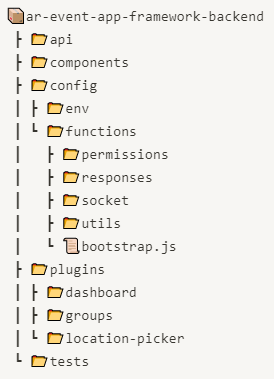
\includegraphics[width=.45\linewidth]{impl/dir_tree_backend.png}
    \caption{Verzeichnisstruktur des Backends}
    \label{fig:impl-backend-structure}
\end{figure}

Der \lstinline[style=code, style=inline]{/api} Ordner beinhaltet die
verschiedenen angelegten APIs des Strapi Projekts. Die meisten der APIs nutzen
hierbei Inhaltstypen (Content-Types). Inhaltstypen werden in Strapi genutzt, um
die Struktur und Art eines Inhalts zu definieren. Die Datenstruktur eines
Inhaltstyps wird dabei durch Attribute festgelegt, welche aus Name, Art und
einstellbaren Einschränkungen bestehen. Strapi stellt drei Arten von
Inhaltstypen bereit: Kollektionen, Einzeltypen und Komponenten. Während
Kollektionen eine Vielzahl von Einträgen beinhalten kann, bestehen Einzeltypen
aus nur einem Eintrag. Komponenten sind hingegen ein wiederverwendbarer
Inhaltstyp, welcher nur in Verbindung mit Kollektionen oder Einzeltypen genutzt
werden kann. Sie sind im \lstinline[style=code, style=inline]{/components}
Verzeichnis wiederzufinden. Die APIs des Systems sind in
\autoref{fig:impl-backend-apis} zu sehen.

\begin{figure}[htpb]
    \centering
    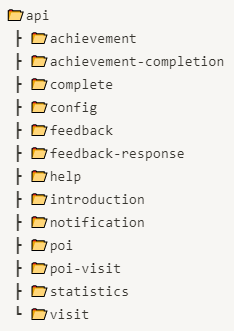
\includegraphics[width=.4\linewidth]{impl/dir_apis.png}
    \caption{Verzeichnisstruktur der Inhaltstypen}
    \label{fig:impl-backend-apis}
\end{figure}

Jede API wird wie folgt unterteilt (s. \autoref{fig:impl-backend-content-type}
zur Verzeichnisstruktur) und anschließend näher erläutert:

\begin{enumerate}
    \setlength{\itemsep}{1em}
    \item \textbf{Konfiguration (/config)} \\
          Zuweisung von Routen zu Kontroller-Funktionen unter Angabe von
          \textit{HTTP-Methode, URL} und \textit{Kontroller-Funktion}.
    \item \textbf{Kontroller (/controllers)} \\
          Enthält Funktionen, welche Anfragen, wie in der Konfiguration
          festgelegt, empfangen, verarbeiten und eine Antwort oder einen Fehler
          zurücksenden.
    \item \textbf{Modelle (/models)} \\
          Legt Datenstruktur und Name des Inhaltstypen fest. Die verfügbaren
          Datentypen werden in \autoref{fig:impl-backend-types} aufgelistet.
          Falls die API keinen Inhaltstypen nutzt, wird dieses Verzeichnis nicht
          benötigt.
    \item \textbf{Dienste (/services)} \\
          Beinhaltet Funktionen, welche zur Wiederverwendung in verschiedenen
          Kontroller-Funktionen gedacht sind. Wird genutzt, um die duplizierten
          Programm-Code zu vermeiden.
\end{enumerate}

\begin{figure}[htpb]
    \centering
    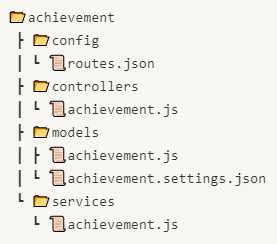
\includegraphics[width=.5\linewidth]{impl/dir_content_type.png}
    \caption{Aufbau eines Inhaltstypen am Beispiel des \textit{Achievement}-Inhaltstypen}
    \label{fig:impl-backend-content-type}
\end{figure}

In der Konfigurationen werden die verschiedenen API Routen des Inhaltstypen
festgelegt. Für jede Route wird die HTTP-Methode, der entsprechende Pfad (z. B.
\textit{/achievements/:id}) und eine Kontroller-Funktion zugewiesen. Bei der
Wahl der HTTP-Methode ist die Funktion der Route zu beachten und sollte der von
\textcite{RFC7231} beschriebenen Semantik folgen. Beispielweise sollte eine
Anfrage, welche lediglich Daten zurückerhalten möchte, die \textit{GET}-Methode
nutzen. Eine Anfrage, welche mir übermittelten Daten einen neuen Eintrag im
System erschafft sollte hingegen die \textit{POST}-Methode nutzen. Alle
voreingestellten Routen sind in \autoref{table:impl-backend-routes} aufgelistet.
Die eingehenden Anfragen werden von der angegebenen Kontroller-Funktion
verarbeitet. \\
Der Kontroller besteht aus Funktionen, welche, wie zuvor beschrieben, ausgeführt
werden, wenn eine für sie hinterlegte Anfrage erhalten wird. In der Anfrage
enthaltene Daten (z. B. abgeschlossenes Abzeichen) werden an die Funktion
übergeben. Innerhalb der Kontroller-Funktion wird die Anfrage verarbeitet und
eine Antwort zurückgesendet. Die Antwort können dabei ein beliebiger
HTTP-Statuscode, binäre Daten oder Daten in JSON-Form sein.
\\
Das Modell bestimmt die Datenstruktur eines Inhaltstypen und nutzt dabei von
Strapi vorgegebene Datentypen (s. \autoref{fig:impl-backend-types}). Jeder
Inhaltstyp setzt sich aus ein oder mehreren Attributen zusammen, welche aus
einem Namen und einem der Datentypen zusammensetzen. Die Attribute können direkt
in der entsprechenden Datei angelegt oder in der Oberfläche von Strapi
festgelegt werden (s. \autoref{fig:impl-backend-content-type-builder}).
\\
Dienste werden genutzt, um duplizierten Code zu vermeiden. Logik, welche an
mehreren Stellen der benötigt wird, kann in einen Dienst geschrieben werden, um
von dort aus in der API benutzt zu werden. Somit fällt der duplizierte Code weg,
was den Code übersichtlicher und leichter anpassbar macht.

\begin{table}[htpb]
    \def\arraystretch{1.25}
    \centering
    \caption{Voreingestellte Routen von Strapi Kollektionen am Beispiel der Abzeichen}
    \label{table:impl-backend-routes}
    \begin{tabular}{lll}
        \uzlhline%
        \uzlemph{Methode} & \uzlemph{Route}              & \uzlemph{Funktion}              \\
        \uzlhline%
        GET               & \textit{/achievements}       & Erhalte alle Abzeichen-Einträge \\
        GET               & \textit{/achievements/:id}   &
        Erhalte Abzeichen-Eintrag mit der angegebenen ID                                   \\
        GET               & \textit{/achievements/count} &
        Erhalte Anzahl der Abzeichen-Einträge                                              \\
        POST              & \textit{/achievements}       &
        Erstellen eines Abzeichen-Eintrags                                                 \\
        DELETE            & \textit{/achievements/:id}   &
        Löschen des Abzeichen-Eintrags mit der angegebenen ID                              \\
        PUT               & \textit{/achievements/:id}   & Verändern des
        Abzeichen-Eintrags mit der angegebenen ID                                          \\
        \uzlhline
    \end{tabular}
\end{table}

\begin{figure}[htpb]
    \centering
    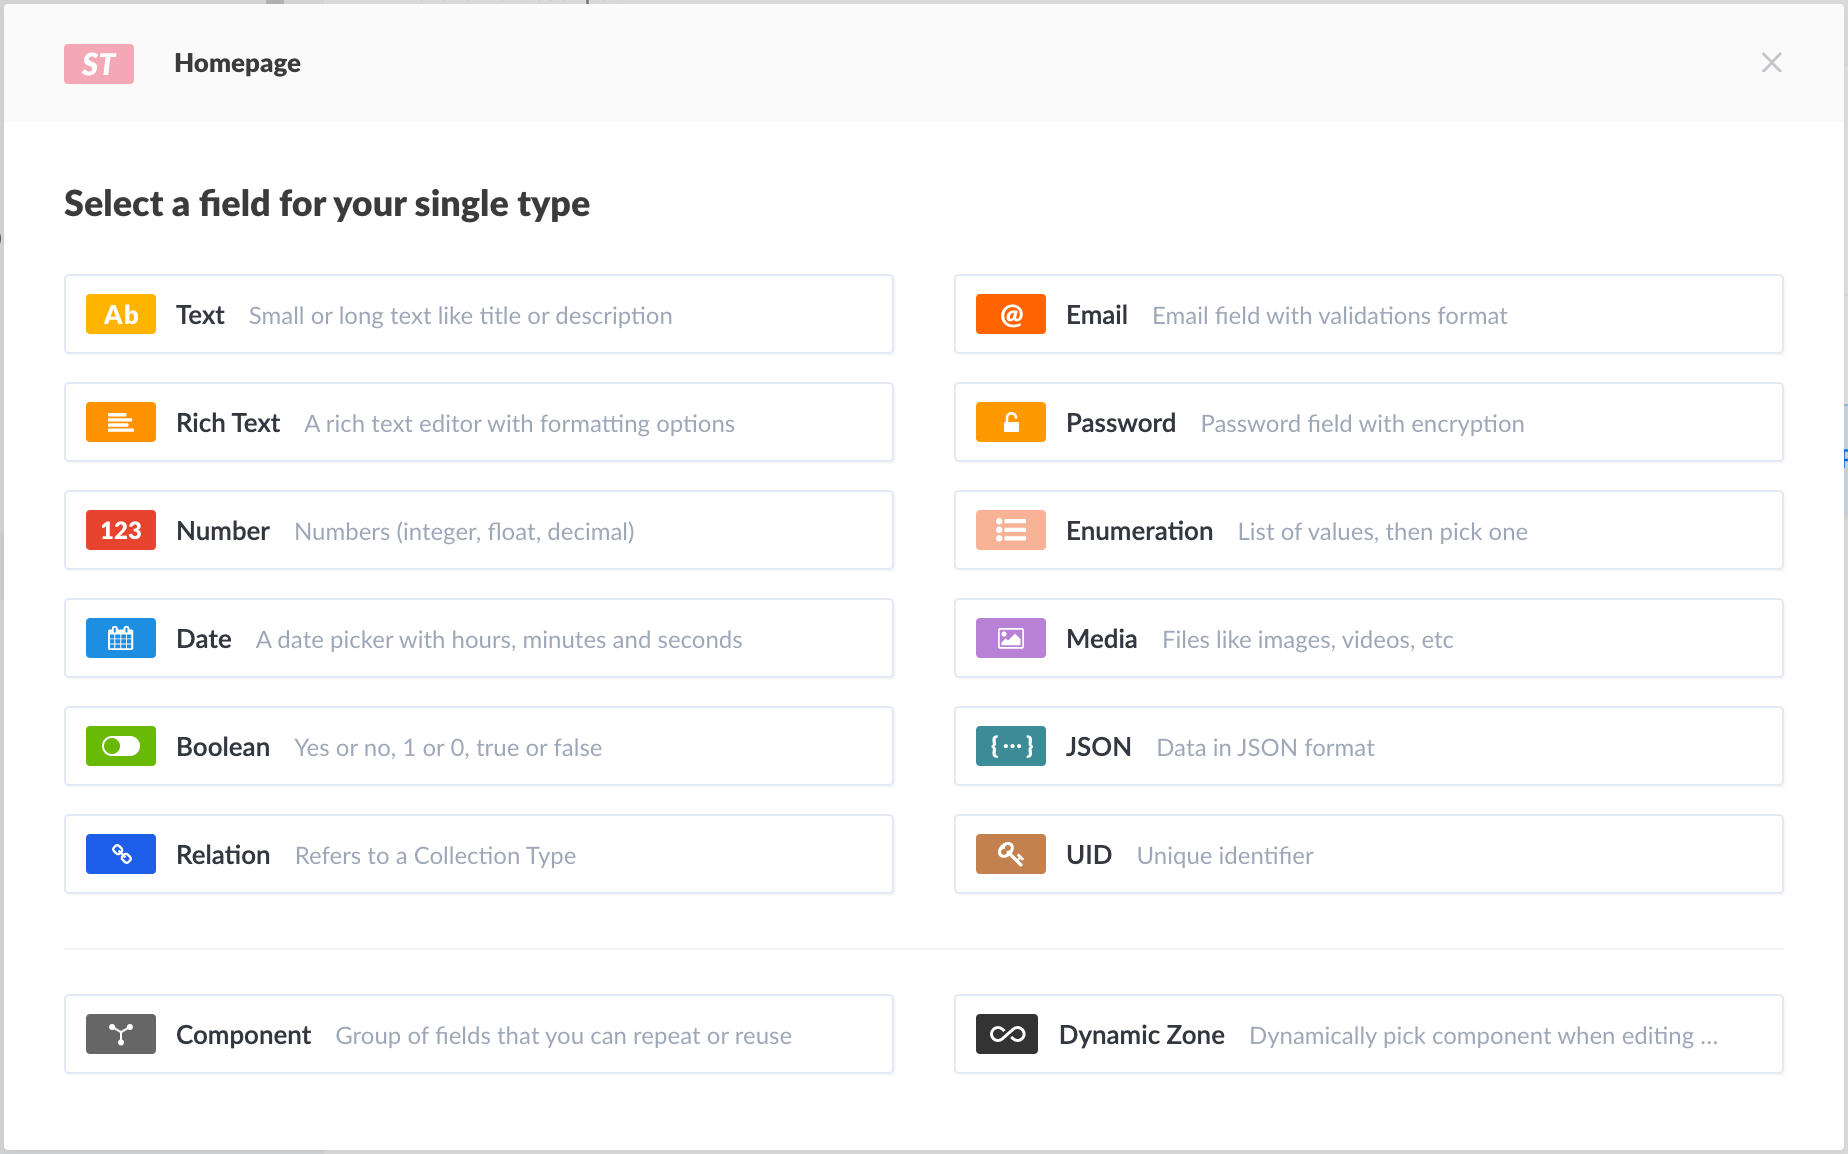
\includegraphics[width=\linewidth]{impl/types.png}
    \caption{Auflistung der verfügbaren Datentypen für Attribute von Inhaltstypen innerhalb Strapis}
    \label{fig:impl-backend-types}
\end{figure}

\begin{figure}[htpb]
    \centering
    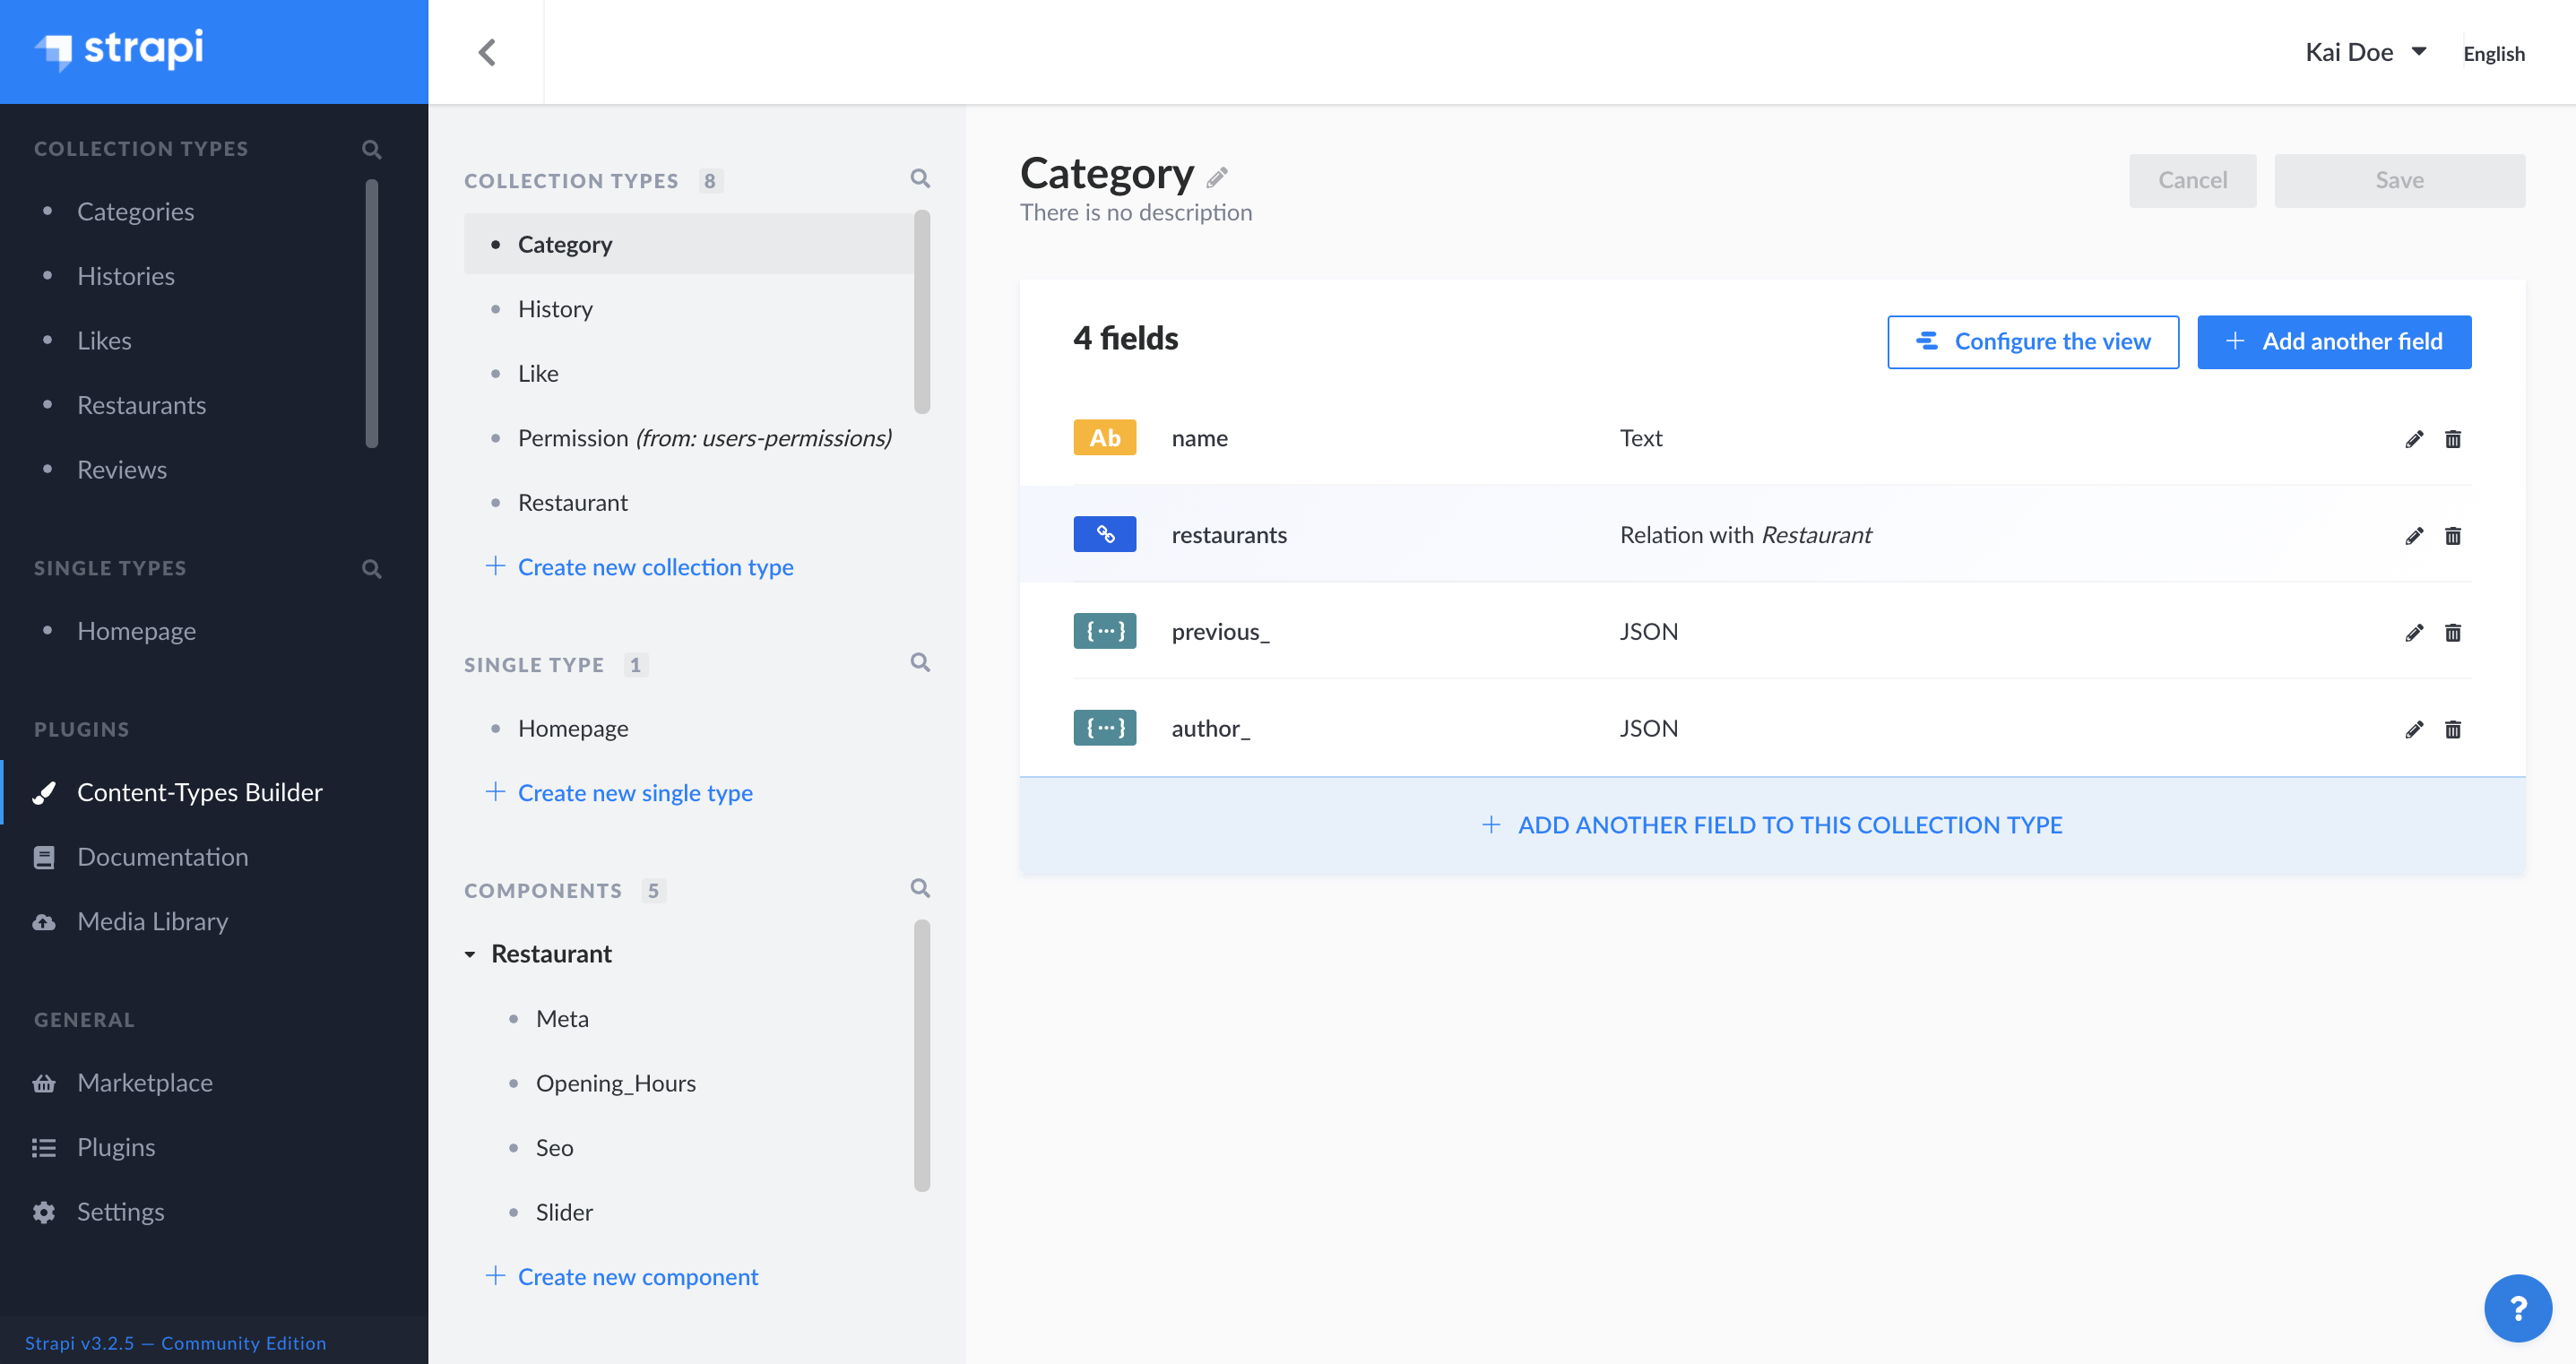
\includegraphics[width=\linewidth]{impl/content-types-builder.png}
    \caption{Oberfläche zum Festlegen der Datenstruktur}
    \label{fig:impl-backend-content-type-builder}
\end{figure}

Das \lstinline[style=code, style=inline]{/config/functions} Verzeichnis des
Projekts enthält Code, welcher zum Start des Systems ausgeführt wird. Die von
der \lstinline[style=code, style=inline]{bootstrap.js} exportierte Funktion
wurde hierbei genutzt, um einen Web-Socket Server zu starten und benötigte
Berechtigungen zu setzen. Auf diese Punkte wird in
\ssecref{ssec:impl-backend-push} genauer eingegangen.

Das \lstinline[style=code, style=inline]{/plugins} Verzeichnis kann genutzt
werden, um Strapi um eigene Module zu erweitern. Möglich ist unter anderem das
Hinzufügen von eigenen Seiten innerhalb der Oberfläche oder die Einbindung einer
eigenen Oberfläche zur Bearbeitung von Attributen. In diesem Projekt sind drei
Plugins zu finden: \textit{groups, dashboard} und \textit{location-picker}. Das
Gruppen-Plugin erfüllt eine Funktion im Backend und wird in
\ssecref{ssec:impl-backend-func} näher erläutert. Das Dash\-board und
Location-Picker-Plugin hingegen werden in \autoref{sec:impl-dashboard}
beschrieben.

Abschließend befinden sich im \lstinline[style=code, style=inline]{/tests}
Verzeichnis Softwaretests, welche genutzt werden, um die korrekte Funktionsweise
der Funktionalitäten, wie in \autoref{sec:concept-func} spezifiziert,
sicherzustellen. Diese sind im Veranstaltungskontext besonders wichtig, da
Fehler während der Veranstaltung im schlimmsten Fall eine komplette
Unterbrechung bedeuten könnten (\anfref{Q30}).

\subsection{Implementierung der Kern-Funktionalitäten} \label{ssec:impl-backend-func}

Nachfolgend wird die Implementierung der Kern-Funktionalitäten des Backends
erläutert, welche aus den Anforderungen aus \autoref{sec:analysis-anf} entnommen
werden. Konkret werden im Folgenden die Implementierung der Stationsbesuche,
Abzeichen und Gruppen erläutert.

Das Besuchen von Stationen erfolgt mithilfe der Übermittlung des Stations-Codes,
welcher aus vier Zeichen, begrenzt auf Zahlen und großen Buchstaben, besteht.
Der Stations-Code ist unabhängig von der ID der Station und kann manuell
festgelegt werden. Dieses Vorgehen ist nötig, da die inkrementellen IDs der
Stations-Kollektion zu einfach zu erraten wären. Zudem können Stations-Codes so
im Nachhinein angepasst werden, sollte z. B. ein Fehler im Druck von QR-Codes
passieren. Eine wichtige Einschränkung bei Stationsbesuchen ist das Verbot von
mehrmaligem Besuchen. Um diese Einschränkung sicherzustellen wurde das Besuchen
von Stationen in einer eigenen \textit{Visit} API realisiert. Die Interaktion
mit der Visit API wird in \autoref{fig:impl-backend-visit-seq} vereinfacht dargestellt.

\begin{figure}[htpb]
    \centering
    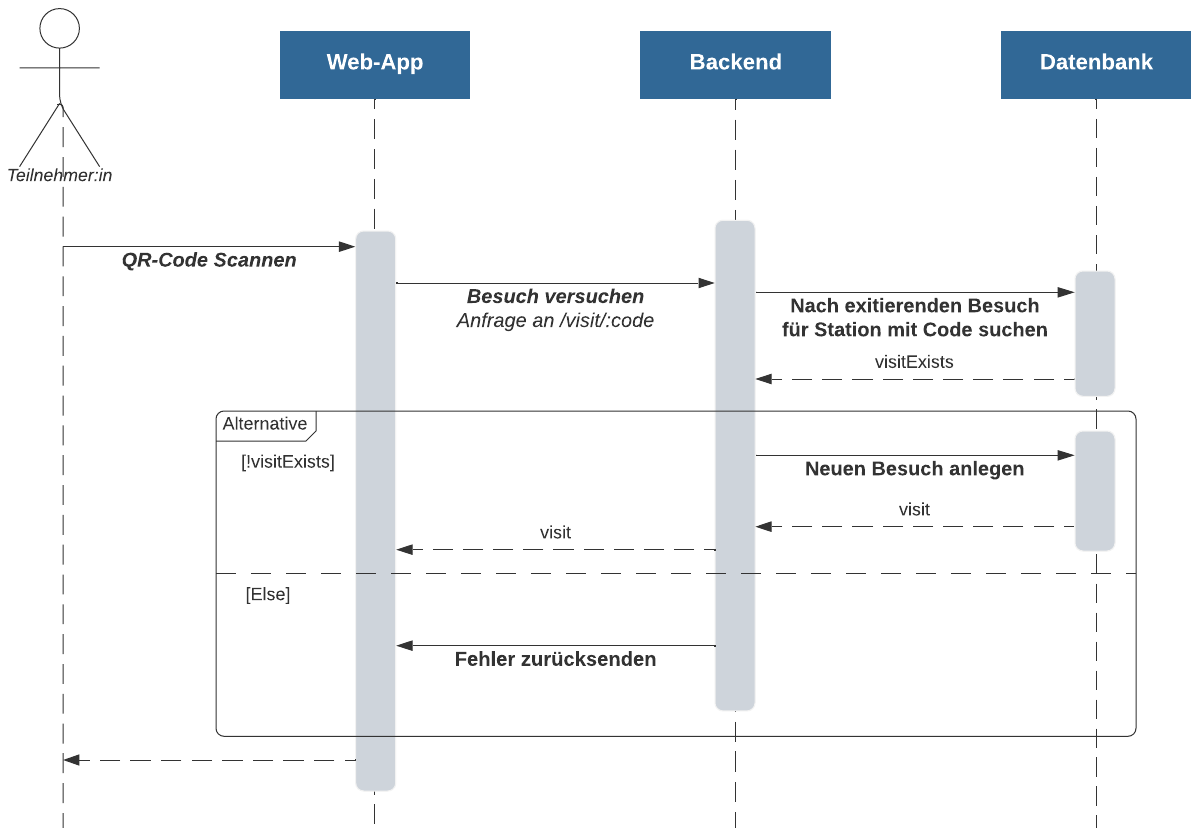
\includegraphics[width=\linewidth]{impl/sequence_visit.png}
    \caption{Interaktion eines Teilnehmenden mit der Visit API}
    \label{fig:impl-backend-visit-seq}
\end{figure}

Um eine Station zu besuchen, wird eine POST Anfrage an \textit{/visit/:code}
abgeschickt, wobei \textit{:code} den Code der Station darstellt. Sollten
Teilnehmende die angegebene Station bereits besucht haben, wird ein
entsprechender Fehlercode zurückgegeben. Andernfalls werden die Daten des
Besuchs, inklusive der Stations-ID, zurückgegeben, um in der Web-App die
Weiterleitung zur entsprechenden Stationsseite zu ermöglichen. Die Datenstruktur
der Stationsbesuche ist in \autoref{fig:impl-backend-visit-data} zu sehen.

\begin{figure}[htpb]
    \centering
    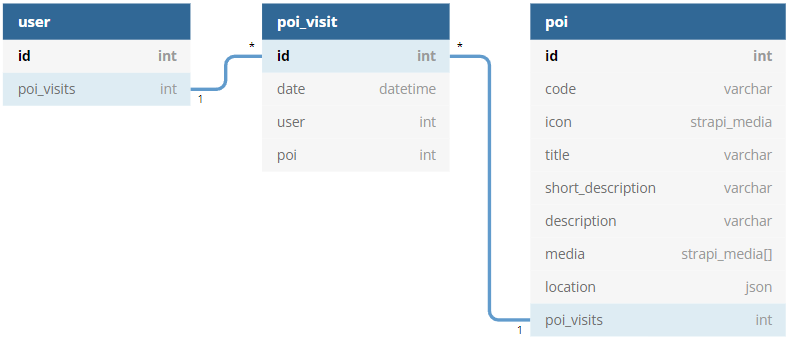
\includegraphics[width=\linewidth]{impl/uml_poi.png}
    \caption{Datenstruktur der Station in Verbindung mit Nutzenden. Intern werden Stationen als \textit{poi} (Point of Interest)
        bezeichnet.}
    \label{fig:impl-backend-visit-data}
\end{figure}

Die Stationsbesuche werden dabei bewusst in einer separaten Tabelle gespeichert,
um die Daten später einfacher zu filtern und das Speichern des Besuch-Zeitpunkts
zu ermöglichen.

Das Abschließen von Abzeichen besitzt, für Bild- und Textabzeichen, einige
Parallelen zum Besuchen von Stationen. Auch hier gilt die Einschränkung, dass
ein bereits eingereichtes Abzeichen nicht erneut eingereicht werden können soll,
solange die Einreichung nicht abgelehnt wurde. Hierfür wurde ebenfalls eine
weitere API hinzugefügt: die \textit{Complete} API. Die Interaktion von
Teilnehmenden mit der Complete API ist in
\autoref{fig:impl-backend-complete-seq} grafisch aufbereitet.

\begin{figure}[ht]
    \centering
    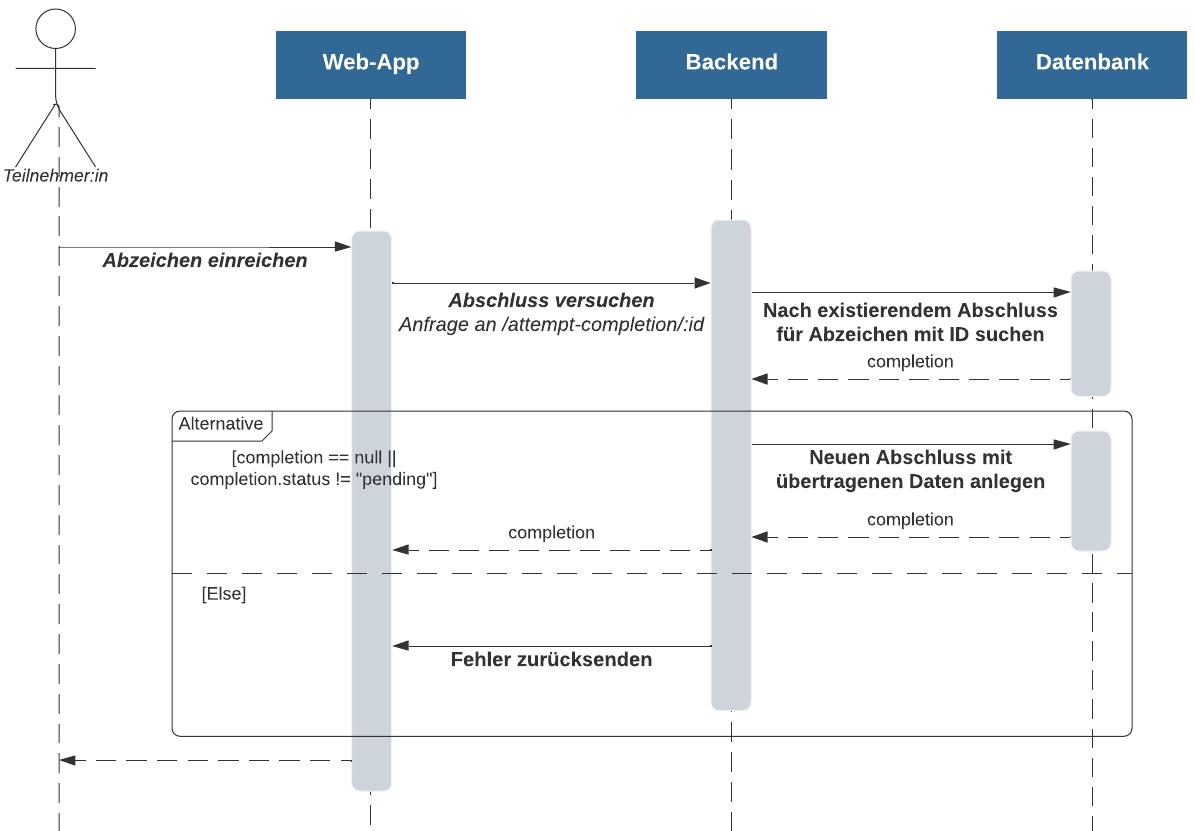
\includegraphics[width=\linewidth]{impl/sequence_completion.png}
    \caption{Interaktion eines Teilnehmenden mit der Complete API}
    \label{fig:impl-backend-complete-seq}
\end{figure}

Um ein Text- oder Bildabzeichen abzuschließen, wird eine POST Anfrage an
\textit{/attempt-completion/:id} abgeschickt, wobei \textit{:id} die ID des
Abzeichens darstellt. Bei vorhandener ausstehender Abgabe wird ein Fehlercode
zurückgegeben. Andernfalls wird die übertragene Einreichung in der Datenbank des
Backends gespeichert. Im Gegensatz zur Visit API wird die Complete API auch von
Veranstaltenden genutzt, um Einreichungen zu bewerten. Über das in
\autoref{sec:impl-dashboard} beschriebene Dashboard können Veranstaltende die
Einreichung akzeptieren oder ablehnen. Daraufhin wird eine Anfrage an
\textit{/complete/:id} bzw. \textit{/dismiss/:id} gesendet, wobei die ID des
Abschlussversuchs übergeben wird (vgl.
\autoref{fig:impl-backend-complete-seq-v}). Wird der Abschlussversuch gefunden
wird der entsprechende Status darin gesetzt. Mögliche Statusangaben sind
„pending“, „denied“ und „accepted“. Der „pending“ Status wird dabei
ausschließlich beim Erstellen des Versuchs verwendet. Diese Logik wird jedoch
nur für Text- oder Bildabzeichen genutzt. Für alle anderen Abzeichen wird die
entsprechende Bedingung im Code überprüft und bei erfüllter Bedingung direkt
ein Eintrag mit „accepted“ für das jeweilige Abzeichen erstellt.

\begin{figure}[htpb]
    \centering
    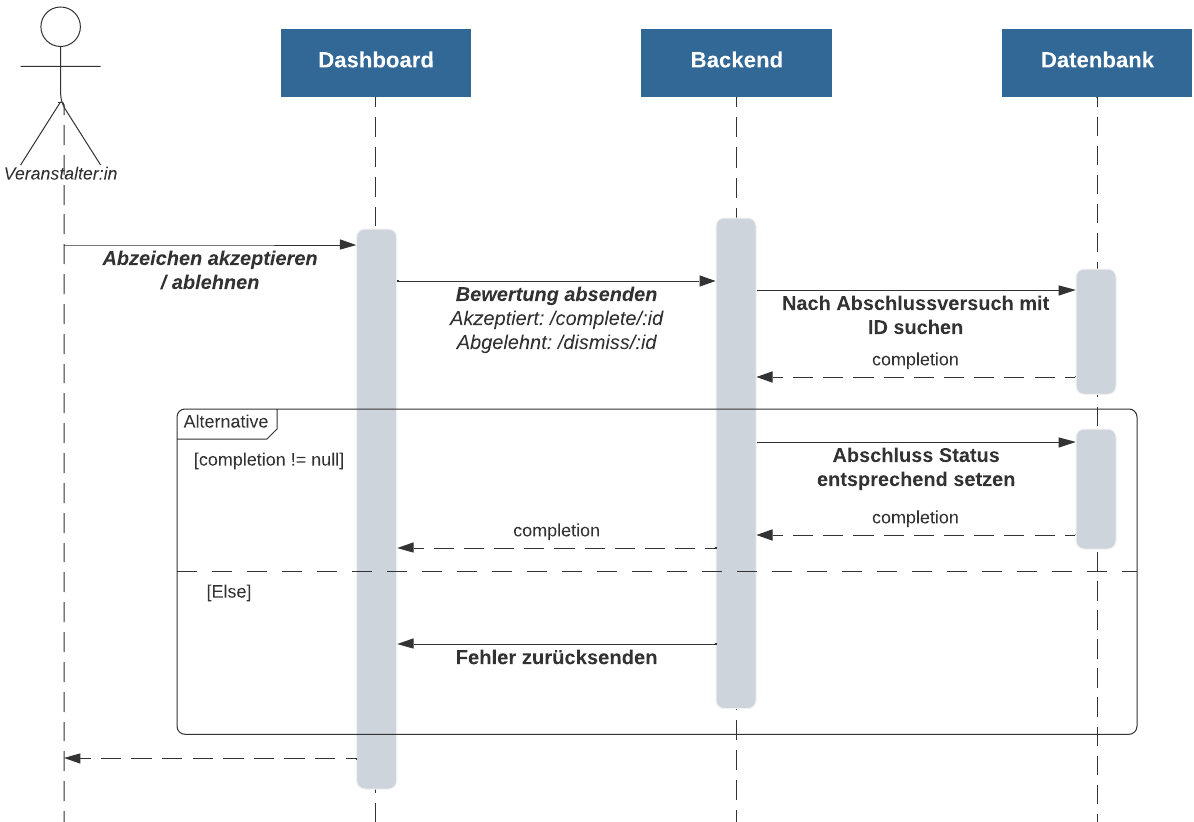
\includegraphics[width=\linewidth]{impl/sequence_completion_v.png}
    \caption{Interaktion eines Veranstaltenden mit der Complete API zum Bewerten einer Einreichung}
    \label{fig:impl-backend-complete-seq-v}
\end{figure}

Ähnlich zur Datenstruktur des Stationsbesuchs werden auch Abzeichen und ihre
dazugehörigen Abschlüsse auf zwei Tabellen aufgeteilt (s. \autoref{fig:impl-backend-completion-data}). Der Grund hierfür ist
ebenfalls die Erfassung der Erstellungs- und Bewertungszeit, sowie die einfache
Durchsuchung.

\begin{figure}[htpb]
    \centering
    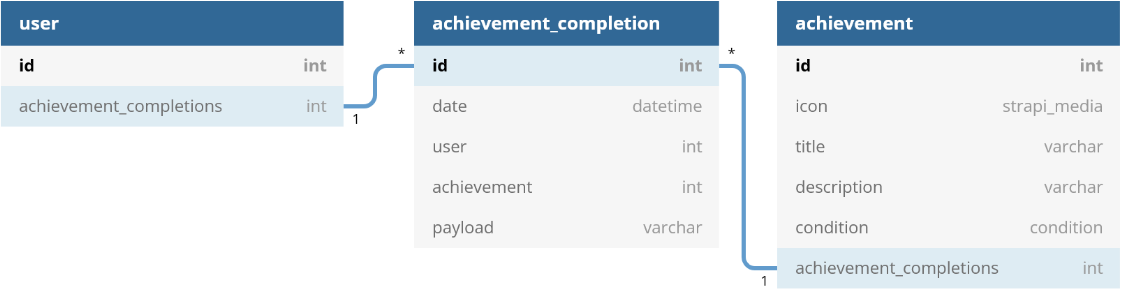
\includegraphics[width=\linewidth]{impl/uml_achievement.png}
    \caption{Datenstruktur der Abzeichen in Verbindung mit Nutzenden}
    \label{fig:impl-backend-completion-data}
\end{figure}

\newpage

Die Gruppen-Funktionalität erweitert Stationsbesuche und Abzeichen, indem
Besuche und Abschlüsse nicht mit Teilnehmenden, sondern analog mit deren Gruppe
verknüpft werden. Sobald ein Gruppenmitglied eine Station oder ein Abzeichen
abschließt, gilt dies somit für alle Mitglieder einer Gruppe. Da die
Gruppen-Funktionalität von Veranstaltenden optional oder ausgeschaltet werden
kann, muss es für Teilnehmende trotzdem möglich sein, diese Aktionen einzeln
auszuführen. Somit ergibt sich die in \autoref{fig:impl-backend-groups-data}
gezeigte Datenstruktur.

\begin{figure}[htpb]
    \centering
    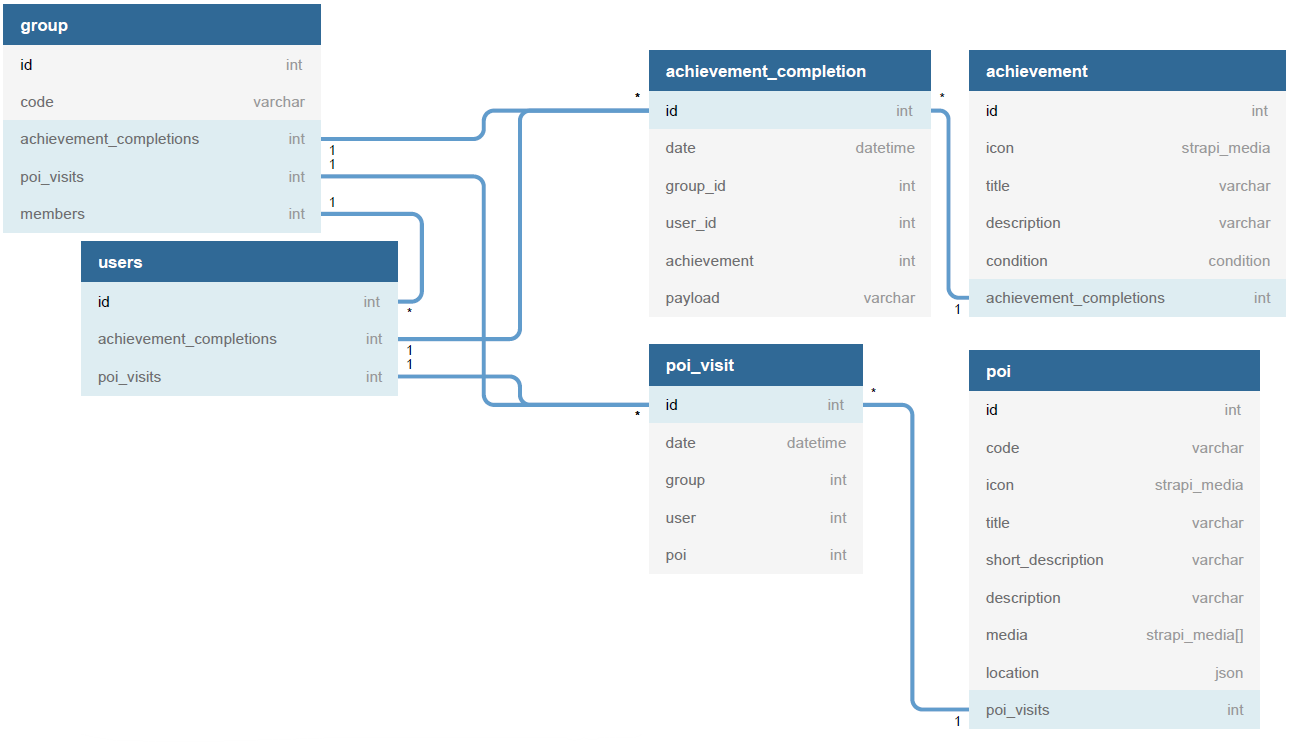
\includegraphics[width=\linewidth]{impl/uml_poi_achievement_group.png}
    \caption{Datenstruktur der Abzeichen und Stationen im Zusammenhang mit Gruppen}
    \label{fig:impl-backend-groups-data}
\end{figure}

Bevor Teilnehmende gemeinsam in einer Gruppe agieren können, müssen sie diese
erstellen oder ihr beitreten. Dies geschieht über eine POST Anfrage an die
\textit{/groups/create} oder \textit{/groups/join} Route. Der
\textit{/groups/create} Route muss zusätzlich der Name der zu erstellenden
Gruppe übermittelt werden, während die \textit{/groups/join} Route den
Gruppen-Code der beitretenden Gruppe benötigt. Abschließend kann die Gruppe auch
wieder verlassen werden, indem eine POST Anfrage an die \textit{/groups/leave}
Route geschickt wird.
\\
Sobald Teilnehmende Mitglied einer Gruppe sind, wird bei Stationsbesuchen und
Abzeichen Einreichungen oder Abschlüssen die Gruppe, statt der Teilnehmenden,
hinterlegt. Gleichzeitig wird beim Auslesen der Besuche und Abschlüsse nicht
mehr nach der Nutzer-ID, sondern der Gruppen-ID gefiltert. Alle
Gruppenmitglieder erhalten somit die neu erstelle Aktion. Eine Einschränkung
dieses Systems ist der temporäre Verlust von Daten bei Beitreten oder Verlassen
einer Gruppe, da jeweils nur Gruppen- bzw. Einzeldaten berücksichtigt werden.
Sobald Teilnehmende ihre Gruppe verlassen, werden wieder Einzeleinträge
angezeigt, da die Gruppeneinträge nicht mehr mit den Teilnehmenden
assoziiert sind. Dies gilt analog auch für das Beitreten einer Gruppe.

\subsection{Implementierung der Push-Benachrichtigungen} \label{ssec:impl-backend-push}
\label{ssec:impl-backend-push}

Gemäß \textit{Ft-V-5} (s. \ssecref{ssec:func-new}) sollen Teilnehmende von
Veranstaltenden jederzeit benachrichtigt werden können. Im Web-Kontext kann dies
über die Web-Push API erfolgen, welche es ermöglicht, auch außerhalb der Nutzung
der Web-App Benachrichtigungen zu erhalten. Jedoch wird die Web-Push API nicht
von Safari auf iOS unterstützt \cite{MDN2021}, weshalb eine Rückfalllösung
gebraucht wird. Unter Beachtung dieser Beschränkungen wurde ein drei-stufiges
Verfahren entwickelt, welches sich aus der Push API und einem Web-Socket Server
zusammensetzt. Im Folgenden werden diese beiden Technologien näher vorgestellt
und ihre Aufgabe und Interaktion im System präsentiert.

Der Web-Push Standard ermöglicht das Versenden und Empfangen von
Push-Benach\-richti\-gungen im Web-Kontext. Ein Endgerät, wie z. B. ein Smartphone
mit Browser, kann durch die Push API einen Push-Dienst abonnieren. Durch das
Abonnieren erhält das Endgerät eine eindeutige URL, welche von einem Server, wie
z. B. dem Backend, genutzt werden kann, um jederzeit Nachrichten an das Endgerät
zu senden. Ein besonderer Vorteil der Web-Push Standards ist das Versenden von
Nachrichten außerhalb der Browsernutzung. Sollten Teilnehmende die Web-App zum
Zeitpunkt des Versendens nicht ausführen, so wird die Nachricht trotzdem
empfangen. Die Funktionsweise der URL birgt jedoch ein Sicherheitsrisiko, da
jeder mit dieser URL beliebige Nachrichten an das entsprechende Endgerät senden
kann. Um diese Sicherheitslücke zu schließen, muss jedes Abonnement
verschlüsselt werden. Dies geschieht mit VAPID-Schlüsseln \cite{VAPID}, wodurch
auf dem Endgerät sichergestellt werden kann, das die Nachricht vom richtigen
Server stammt.

Web-Sockets hingegen sind für die Echtzeit-Kommunikation zwischen Endgerät und
Server gedacht. Sie ermöglichen das Senden und Empfangen von Nachrichten in
beide Richtungen. Somit kann das Endgerät, im Gegensatz zum Web-Push Standard,
auch Nachrichten an den Server schicken. Hierzu wird eine dauerhafte Verbindung
mit dem Server aufgebaut, welche jedoch mit dem Schließen der Web-App abbricht.
Im Vergleich zum Web-Push Standard eigenen sich Nachrichten über Web-Sockets
somit nur während der Nutzung der App. Jedoch werden für Web-Sockets keine
weiteren Verschlüsselungsmethoden, neben der Nutzung von HTTPS, benötigt. Zudem
vereinfachen JavaScript-Bibliotheken wie Socket.IO\footnote{\url{https://socket.io/}},
welche in dieser Arbeit verwendet wurde, die Nutzung von Web-Sockets und
verwenden intern weitere Methoden um eine stabile Verbindung über eine
breite Auswahl an Geräten zu garantieren \cite{SocketIO2022}.


Basierend auf den Fähigkeiten der beiden vorgestellten Technologien wird ein
drei-stufiges Verfahren zur Benachrichtigung entwickelt, welches in
\autoref{fig:impl-backend-push} präsentiert wird. Wenn Veranstaltende eine
Nachricht versenden, wird zunächst das Versenden mit Web-Push versucht. Sollte
dies fehlschlagen, wird die Nachricht stattdessen über eine Web-Socket
Verbindung versendet. Falls auch dies fehlschlägt, wird die Nachricht im
Nutzerprofil gespeichert. Sobald Teilnehmende sich wieder mit dem Server
verbinden, wird dieser Vorgang erneut versucht. Allerdings wird die Nachricht in
diesem Fall verworfen, sollte die Nachricht weder per Web-Push noch Web-Sockets
versendet werden können (s. \autoref{fig:impl-backend-push-connect}).

\begin{figure}[htpb]
    \centering
    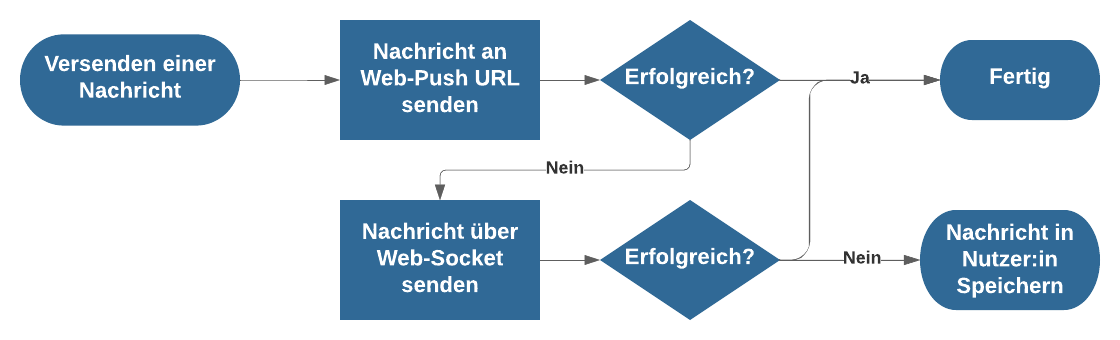
\includegraphics[width=\linewidth]{impl/flow_push.png}
    \caption{Verfahren zum Versenden von Benachrichtigungen an Teilnehmende}
    \label{fig:impl-backend-push}
\end{figure}

\begin{figure}[htpb]
    \centering
    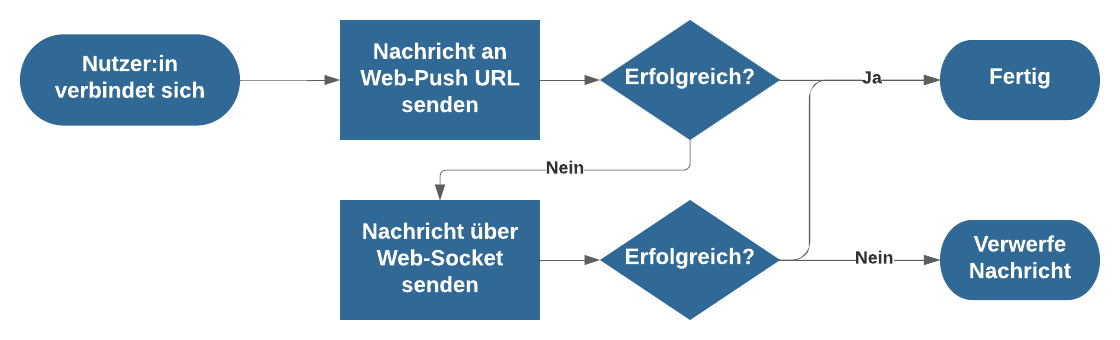
\includegraphics[width=\linewidth]{impl/flow_push_connect.png}
    \caption{Verfahren bei ausstehenden Benachrichtigungen}
    \label{fig:impl-backend-push-connect}
\end{figure}

\subsection{Implementierung der Feedback-Funktionalität}

Die Feedback-Funktionalität baut auf der Implementierung der
Push-Benachrichtigungen auf. Sobald Veranstaltende eine neue Feedback-Anfrage
verschicken, wird diese an alle Teilnehmende über das in
\ssecref{ssec:impl-backend-push} beschriebene Verfahren gesendet. Dabei wird
jede Feedback-Anfrage mit einer eindeutigen ID versehen, um die Antworten später
noch zur jeweiligen Anfrage zuordnen zu können. Die Datenstruktur des
Feedback-Systems wird in \autoref{fig:impl-backend-feedback-data} dargestellt.
Jede verschickte Feedback-Anfrage ist hierbei ein Eintrag in der
\textit{feedback} Tabelle, während die Antworten der Teilnehmenden als Einträge
in der \textit{feedback-response} Tabelle gespeichert werden. Hierzu wird die
Antwort als POST Anfrage an \textit{/feedback/respond} gesendet.

\begin{figure}[htpb]
    \centering
    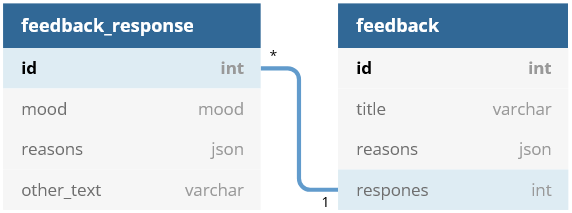
\includegraphics[width=0.6\linewidth]{impl/uml_feedback.png}
    \caption{Datenstruktur des Feedback-Systems}
    \label{fig:impl-backend-feedback-data}
\end{figure}

%\subsection{Softwarequalität}

% - Aussagekräftige Fehlermeldungen ->
% - Softwaretests

\section{Implementierung des Frontends}

Dieser Abschnitt präsentiert bedeutendsten technischen Aspekte des Frontends.
Zunächst wird der Aufbau des Projekts und die Nutzung des Vue CLI betrachtet.
Daraufhin wird die Komponentenstruktur am Beispiel der interaktiven Karte näher
erläutert. Abschließend werden das native App-Erlebnis und die
Fortschrittsspeicherung aufgegriffen.

\subsection{Struktur mit Vue CLI} \label{ssec:impl-frontend-structure}

Zur Erstellung und Verwaltung des Projekts wurde das \textit{Vue CLI} genutzt.
Vue CLI ist ein Kommandozeilenprogramm, welches die Einrichtung und Verwaltung
von komplexeren Vue Projekten stark vereinfacht. Das Erstellen eines Projekts
erfolgt nach Installation des Vue CLI durch den Befehl \lstinline[style=code,
    language=bash, style=inline]{vue create <projekt-name>}. Während der Erstellung
des Projekts können zusätzliche Plugins ausgewählt werden, welche einige
Vue-spezifische oder allgemeine Funktionalitäten hinzufügen. Für dieses Projekt
wurden die Plugins aus \autoref{table:impl-frontend-vuecli-plugins} zur
Installation ausgewählt. Die Struktur des Vue-Projekts dieser Arbeit wird in
\autoref{fig:impl-frontend-vuecli-dir} präsentiert. Die fettgedruckten
Verzeichnisse sind nicht durch das Vue CLI generiert worden, sondern wurden
manuell erstellt. Nachfolgend wird die Struktur näher erläutert.

\begin{table}[htpb]
    \caption{Gewählte Vue CLI Plugins und ihre Funktion}
    \label{table:impl-frontend-vuecli-plugins}
    \begin{threeparttable}[t]
        \def\arraystretch{1.25}
        \centering
        \begin{tabularx}{\textwidth}{lX}
            \uzlhline%
            \uzlemph{Plugin}     & \uzlemph{Funktion}                                                      \\
            \uzlhline%
            \textbf{TypeScript}\tnote{1}  & Ermöglicht die Nutzung von TypeScript innerhalb
            eines Vue Projekts. TypeScript ergänzt JavaScript um eine Syntax für
            Datentypen, welche besser Vorschläge in Entwicklungsumgebungen
            ermöglicht und vorzeitig Fehler aufzeigen kann.                                                \\
            \textbf{PWA Support} &
            Generiert alle nötigen Dateien und Konfigurationen, welche für die
            Nutzung einer PWA benötigt werden. Zudem wird die Anpassung von PWAs an
            die eigenen Bedürfnisse vereinfacht.                                                           \\
            \textbf{Router}      &
            Fügt \textit{vue-router}\tnote{2}und seine benötigten Dateien zum Projekt hinzu.
            Vue-router ermöglicht das Anlegen von und Navigieren zu mehreren (Unter-)Seiten
            innerhalb der Web-App.                                                                         \\
            \textbf{Vuex}\tnote{3}        & Ergänzt das Projekt um einen zentralisierten
            Speicher, welcher das einfache Verwalten von globalen Zuständen
            ermöglicht. Dies umfasst Daten wie z. B. den Standort des Nutzers,
            welcher in mehreren Teilen der App benötigt wird.                                              \\
            \uzlhline
        \end{tabularx}
        \vspace{-0.75cm}
        \begin{tablenotes}
            \item [1] \url{https://www.typescriptlang.org/}
            \item [2] \url{https://router.vuejs.org/}
            \item [3] \url{https://vuex.vuejs.org/}
        \end{tablenotes}
    \end{threeparttable}
\end{table}


\begin{figure}[htpb]
    \centering
    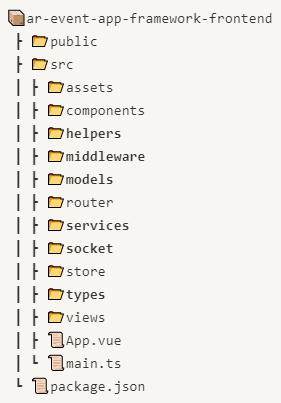
\includegraphics[width=0.45\linewidth]{impl/dir_frontend.png}
    \caption{Verzeichnisstruktur des Frontends mit Vue CLI}
    \label{fig:impl-frontend-vuecli-dir}
\end{figure}

Projekte, welche mit dem Vue CLI erstellt werden, gliedern sich im wesentlichen
in zwei Ordner: \textit{public} und \textit{src}. Der \textit{public} Ordner
beinhaltet statische Datein, wie z. B. die \textit{index.html}, welche als
Template für die Vue-App genutzt wird. Weitere Dateien, die im \textit{public}
Ordner gefunden werden können, sind \textit{robots.txt}, welche
Suchmaschinen Hinweise zur Indexierung der Seite geben, und
\textit{favicon.ico}, welches vom Browser als Tab-Icon verwendet wird.

Der \textit{src} Ordner beinhaltet Code der eigentlichen Vue-App und ist in
weitere Ordner eingeteilt. Diese Ordner unterteilen den Code der App in seine
Aufgaben, wie z. B. das Anzeigen von Inhalten oder Abfragen von externen Daten.
Der Einstiegspunkt der App bilden hierbei die \textit{main.ts} und
\textit{App.vue}. In ihnen wird die Vue-App initialisiert und das Grundlegende
Layout festgelegt. Plugins und globale Stylesheets werden hierbei in der
\textit{main.ts} eingebunden. Die \textit{App.vue} stellt hingegen die oberste
Vue-Kompontente dar, in welcher die gesamte Web-App dargestellt wird. Dauerhaft
sichtbare Element, wie die Navigationsleiste, wurden hier angelegt, um
duplizierten Code zu vermeiden.

Alle Ansichten befinden sich im \textit{views} Ordner. Die Ansichten selber
nutzen meist mehrere Komponenten aus dem \textit{components} Ordner. Dies
ermöglicht das Wiederverwenden von Komponenten in mehreren Ansichten, wodurch
duplizierter Code vermieden werden kann. Zudem ermöglichen Komponenten das
Abkapseln bestimmter Logik, um die Vue-App klarer zu strukturieren. Bilder und
andere Dateien, welche fest in der App eingebunden werden, sind im
\textit{assets} Ordner zu finden.

Die einzelnen Ansichten lassen sich jeweils über ihre URL aufrufen. Hierzu wird
diese, sowie einige weitere Optionen, innerhalb der \textit{vue-router}
Konfiguration im \textit{router} Ordner festgelegt. Zudem beinhaltet der
\textit{store} Ordner den im vorherigen Abschnitt erwähnten, globalen
\textit{Vuex} Speicher. Dieser wird genutzt, um Daten wie die Position der
Teilnehmenden oder Einstellungen abzuspeichern, da diese an vielen Stellen der
Vue-App benötigt oder verändert werden.

Alle bisher erwähnten Verzeichnisse und Dateien werden automatisch durch das Vue
CLI generiert. Zur bessern Übersichtlichkeit wurden weitere Ordner angelegt, um
eigene Funktionen nach Aufgabe zu gruppieren. Die \textit{models} und
\textit{services} Ordner beinhalten Funktionen zur Abfrage von Daten aus dem
Backend. Hierbei werden in \textit{models} die Typen der verschiedenen
Datenstrukturen des Backends repliziert. Die Anfrage-Funktionen des
\textit{services} Verzeichnisses nutzen diese Typen, um in der Vue-App die
Typisierung von externen Anfragen zu erlauben. Somit können Fehler in der
Nutzung der abgefragten Daten schneller erkannt werden. Der \textit{helpers}
Ordner enthält einige allgemeinere, hilfreiche Funktionen, welche in vielen
Teilen der Vue-App genutzt werden. Im \textit{middleware} Ordner sind sogenannte
„Middlewares“ zu finden. In diesem Kontext handelt es sich hierbei um
Funktionen, welche bei der Navigation zwischen Ansichten aufgerufen werden, um
z. B. zu kontrollieren, ob Teilnehmende authentifiziert sind. Das \textit{types}
Verzeichnis enthält TypeScript Typen für Pakete, welche keine Typen besitzen.
Somit können auch für diese Pakete die Vorteile von TypeScript genutzt werden.


\urldef\vuemixin\url{https://vuejs.org/guide/reusability/composables.html#comparisons-with-other-techniques}

Abschließend verfügt Vue.js seit der Version 3.0 über zwei verschiedene Arten,
den Aufbau von Komponenten organisieren: die Composition API und die Options
API. Die Options API ist hierbei die traditionelle Art Vue Komponenten zu
organisieren und war vor Version 3.0 die einzige Möglichkeit.
\autoref{fig:impl-frontend-vue-api-options} zeigt eine Beispiel-Komponente,
welche die Options API nutzt. Hierbei wird die Komponente nach der Art ihrer
Inhalte, der sogenannten „Options“, strukturiert. Alle Methoden, Variablen und
übergebenen Werte werden jeweils gruppiert angegeben. Diese Art der
Strukturierung ermöglicht einen einheitlichen Aufbau über große Projekte. Jedoch
besitzt sie auch einige große Nachteile, wenn Teile der Komponente extrahiert
und wiederverwendbar gestaltet werden sollen\footnote{\vuemixin}.

\begin{figure}[htpb]
    \centering
    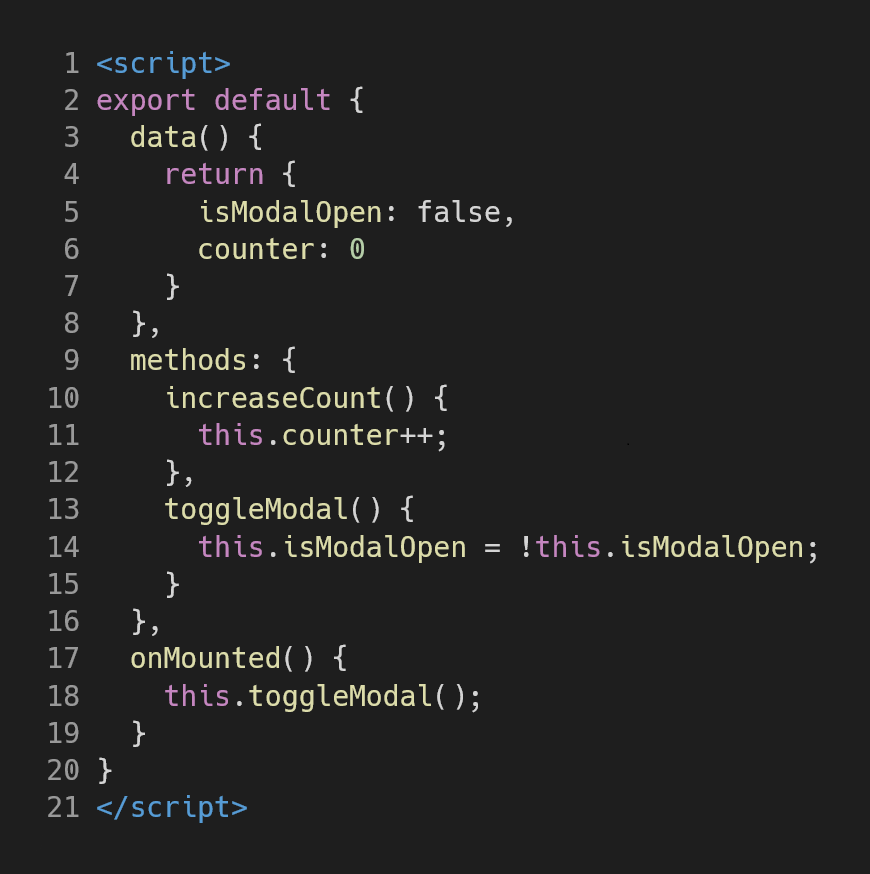
\includegraphics[width=0.65\linewidth]{impl/code_options.png}
    \caption{Beispiel-Komponente mit der Options API (Nur Script)}
    \label{fig:impl-frontend-vue-api-options}
\end{figure}

\urldef\vuecomp\url{https://vuejs.org/guide/extras/composition-api-faq.html#why-composition-api}
\urldef\vuets\url{https://vuejs.org/guide/extras/composition-api-faq.html#better-type-inference}

Die Composition API wurde konzipiert um dieses Problem und weitere zu beheben.
Anstatt Optionen anzugeben, werden die gewünschten Funktionalitäten importiert
und in beliebiger Struktur genutzt. Somit kann der Code nach seiner Funktion
gruppiert werden. Zum Vergleich ist die Composition API Version der
Beispiel-Komponente auf \autoref{fig:impl-frontend-vue-api-composition} zu
sehen. Zusätzlich wird TypeScript in der Composition API besser
unterstützt\footnote{\vuets}. In dieser Arbeit wird, aufgrund der vorgestellten
Vorteile und Empfehlung der offiziellen Dokumentation\footnote{\vuecomp}, die
Composition API genutzt.

\begin{figure}[htpb]
    \centering
    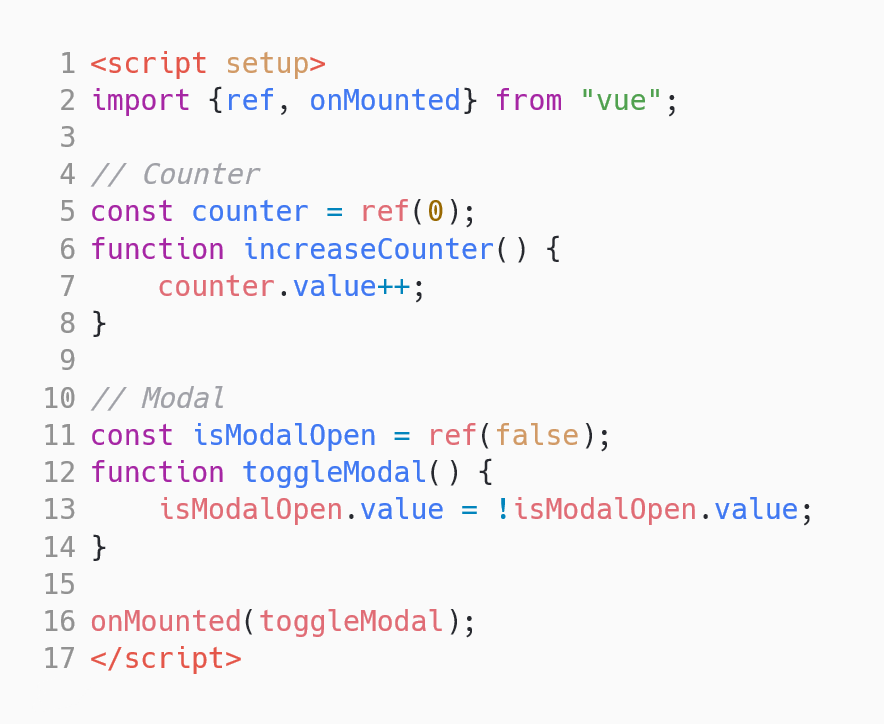
\includegraphics[width=0.65\linewidth]{impl/code_composition.png}
    \caption{Beispiel-Komponente mit der Composition API (Nur Script)}
    \label{fig:impl-frontend-vue-api-composition}
\end{figure}

%\subsection{API-Kommunikation}

\subsection{Komponentenstruktur}

Wie in \ssecref{ssec:impl-frontend-structure} beschrieben, besteht die Vue-App
aus einer Hierarchie an Ansichten und Komponenten. Im Folgenden wird am Beispiel
der interaktiven Karte aufgezeigt, wie diese Strukturen entwickelt wurden.
Hierfür wurde die Hierarchie der interaktiven Karte vereinfacht grafisch
dargestellt (s. \autoref{fig:impl-frontend-components-structure}).

\begin{figure}[htpb]
    \centering
    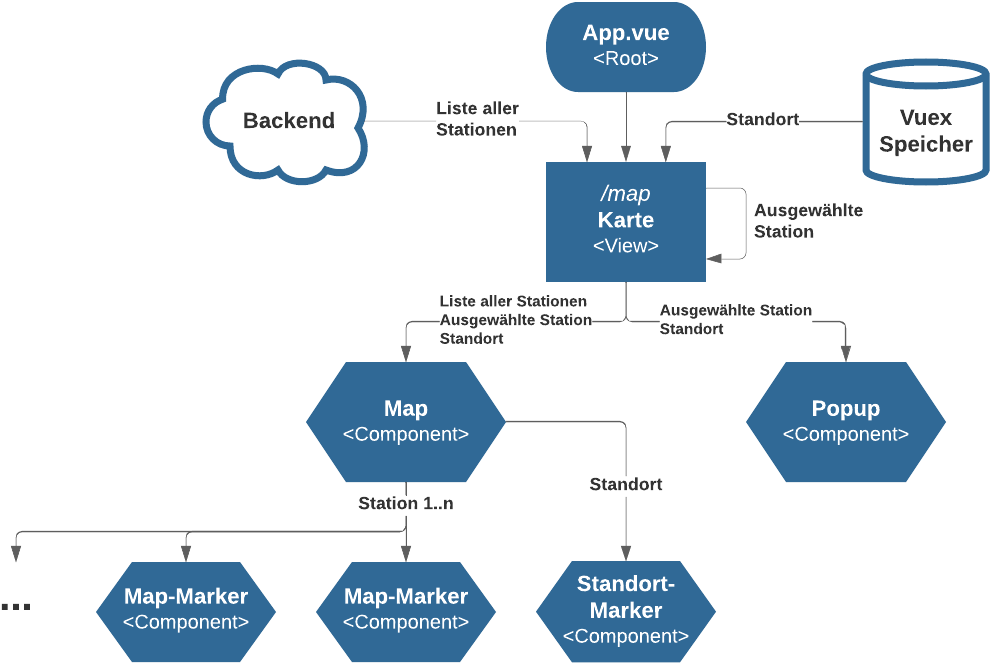
\includegraphics[width=\linewidth]{impl/component_map.png}
    \caption{Vereinfachter hierarchischer Aufbau der interaktiven Karte}
    \label{fig:impl-frontend-components-structure}
\end{figure}

Den Startpunkt der Hierarchie bildet, wie bereits in
\ssecref{ssec:impl-frontend-structure} beschrieben, die \textit{App.vue}. Im
Beispiel ist zurzeit die Karten-Ansicht ausgewählt, welche sich im
\textit{views} Verzeichnis befindet (s. \autoref{fig:impl-frontend-dirs} links,
\textit{Map.vue}). Diese wird durch ihren zugehörigen Pfad \textit{/map}
erreicht, welcher so im vue-router definiert wurde. Da die Aufgabe der Karte das
Anzeigen aller Stationen ist, fragt die Karten-Ansicht eine Liste aller
Stationen vom Backend an. Zusätzlich wird der Standort aus dem Vuex Speicher
benötigt, welcher zur Berechnung der Distanz und dem Anzeigen auf der Karte
genutzt wird. Intern überwacht die Karten-Ansicht zudem, welche Station aktuell
ausgewählt ist.

\begin{figure}[htpb]
    \centering
    \begin{minipage}{.5\textwidth}
        \centering
        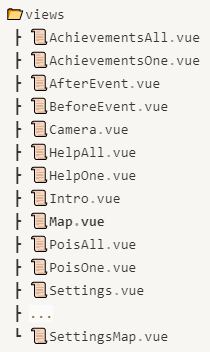
\includegraphics[width=.7\linewidth]{impl/dir_frontend_views.png}
    \end{minipage}%
    \begin{minipage}{.5\textwidth}
        \centering
        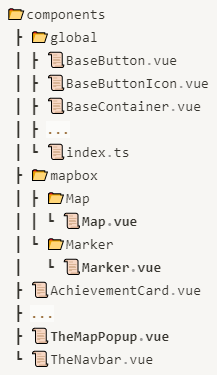
\includegraphics[width=.7\linewidth]{impl/dir_frontend_components.png}
    \end{minipage}
    \caption{Ausschnitt der Inhalte der \textit{views} und \textit{components}
    Verzeichnisse. Die Strukturierung und Benennung der Inhalte folgt dem Vue
    Style Guide \cite{You2022b}}
    \label{fig:impl-frontend-dirs}
\end{figure}

Diese Daten werden nach Bedarf an die Komponenten der Ansicht weitergegeben. Die
Karten-Ansicht besteht hierbei im Wesentlichen aus zwei Komponenten: der
interaktiven Karte (\textit{mapbox/Map/Map.vue}) und einem Pop-up
(\textit{TheMapPopup.vue}), welche sich im \textit{components} Verzeichnis
befinden (s. \autoref{fig:impl-frontend-dirs} rechts). Wie
\autoref{fig:impl-frontend-components-structure} zu entnehmen ist, erhält die
\textit{Map}-Komponente alle drei Daten der Karte-Ansicht, während das Pop-up
lediglich die ausgewählte Station und den Standort übergeben bekommt. Die
interaktive Karte ist hierbei nur für das Anzeigen der Karte, nicht aber der
Stationsicons, verantwortlich.

Um die Stationen anzuzeigen wird intern die Map-Marker Komponente genutzt. Für
jede in der Liste vorhandene Station wird eine Map-Marker Komponente
instanziiert und mit den Daten der jeweiligen Station versorgt. Hieraus werden
Icon und Position der Station entnommen, um diese korrekt anzuzeigen. Zudem
übernimmt die Map-Marker Komponente die Anpassung des Icons, falls die Station
ausgewählt ist oder bereits besucht wurde. Der Standort wiederum benötigt diese
Logik nicht und wird separat verwendet.

Die Pop-up Komponente nutzt die übergebene, ausgewählte Station um ihre
Informationen wie Titel und Beschreibung anzuzeigen. Zusätzlich wird der
Standort verwendet, um die Distanz zur ausgewählten Station zu berechnen und
anzuzeigen. Intern setzen sich diese Komponenten noch aus weiteren Komponenten
zusammen, wie z. B. einer Icon-Komponente. Zur Übersichtlichkeit und
Verständlichkeit wurde dieses Beispiel jedoch vereinfacht.

Dieser hierarchische Aufbau und die Weitergabe der Daten an untergeordnete
Komponenten findet sich in der gesamten Vue-App wieder. Hierdurch können
Komponenten im System an vielen Stellen wiederverwendet werden, was
Entwicklungszeit spart und unterschiedliche Fehler in sich widerholendem Code
vermeidet.

\subsection{Natives App-Erlebnis}
% Enkodierung des UI-Zustandes in der URL

Aufgrund der technischen Limitierungen ist eine native App im Rahmen dieser
Bachelorarbeit nicht möglich (s. \ssecref{ssec:analysis-old-tech}). Um
Teilnehmenden trotzdem ein möglichst natives App-Erlebnis zu ermöglichen, wurden
einige Maßnahmen eingesetzt. Nachfolgend wird erläutert wie der
\textit{vue-router} und die \textit{PWA}-Funktionalität hierfür genutzt wurden.

Traditionelle Webseiten müssen für jede aufgerufene Seite eine neue Anfrage an
den jeweiligen Server stellen. Dies ist mit meist mit einer längeren Wartezeit
verbunden. Jedoch werden Interaktionen bei Wartezeiten von mehr als einer
Sekunde bereits die Gedankengänge von Nutzenden unterbrochen und die Interaktion
fühlt sich wahrnehmbar verzögert an \cite{Nielsen1994b}. Um dieses Problem zu
umgehen, verwendet diese Arbeit das \textit{vue-router} Paket. Im Gegensatz zu
traditioneller Navigation zwischen Seiten wird bei der Verwendung von vue-router
der Großteil der Navigation mithilfe von JavaScript übernommen.

Anstatt bei jedem Aufruf erneut die HTML-Seite zu laden, wird nur noch eine
HTML-Seite angefragt, welche alle benötigten Daten der restlichen Anwendung
enthält. Bei jedem Seitenwechsel wird der Inhalt der Seite mithilfe des
JavaScript-Codes ausgetauscht. Dies verkürzt die Ladezeit und erlaubt es, die
Übergänge zwischen den Seiten nach Bedarf anzupassen. Das Prinzip dieser
gebündelten Seite nennt sich \textit{Singe-Page-Application (SPA)}.

Ein Nachteil von SPAs ist die Größe der Dateien beim ersten Aufruf. Um dieses
Problem zu minimieren, werden die Dateien meist stark komprimiert. Zudem lassen
sich verschiedene Teile der SPA nach Bedarf aufteilen und nachladen. Auch wenn
hier wieder eine Anfrage an den Server gestellt werden muss, ist dies schneller
als das Laden einer kompletten Seite. Zudem kann hier die PWA-Funktionalität
genutzt werden.

Progressive Web-Apps ermöglichen u. a. das Vorladen und Speichern von Webseiten,
um diese auch offline nutzen zu können. Hierzu werden JavaScript \textit{Service
Worker} genutzt. Service Worker sind JavaScript Prozesse, welche auf einem
separaten Thread ausgeführt werden und auch nach dem Schließen der Seite noch
aktiv sind. In ihnen können Dateien festgelegt werden, welche beim ersten Aufruf
der Seite direkt geladen und gespeichert werden sollen. Obwohl dies eine längere
Ladezeit zum ersten Aufruf bedeutet, werden alle weiteren Navigationen
zusätzlich beschleunigt, während die übertragenen Daten minimiert werden.
Besonders die Minimierung der übertragenen Daten spielt eine wichtige Rolle im
mobilen Kontext durch meist begrenzte Datenvolumen in Mobilfunkverträgen.

Zudem werden Service Worker benötigt, um Push-Benachrichtigungen zu empfangen.
Die Notifications
API\footnote{\url{https://developer.mozilla.org/en-US/docs/Web/API/Notifications_API}}
erlaubt es native Benachrichtigungen zu erstellen, welche das native
App-Erlebnis födern.

\subsection{Persistente Nutzerdatenspeicherung}

Da die Nutzung der App sich über mehrere Wochen erstrecken kann (s.
\autoref{sec:analysis-context}), ist die sichere Speicherung der Fortschritte
der Teilnehmenden ein wichtiger Faktor. Um dies zu gewährleisten werden die
Fortschrittsdaten auf dem Server in einem Nutzerprofil gespeichert. Dieses
Profil wird automatisch mit dem Akzeptieren der Datenschutzerklärung erstellt.
Da Teilnehmende keine identifizierenden Daten, wie z. B. eine E-Mail Adresse,
angeben müssen, wird stattdessen eine eindeutige ID generiert. Diese ID basiert
auf dem Browser Fingerprint der Teilnehmenden. Der Browser Fingerprint setzt
sich aus vielen auslesbaren Eigenschaften des Browsers zusammen. Hierzu gehören
z. B. die Bildschirmgröße, installierten Schriftarten, genutzte Hardware oder
Implementierungsunterschiede der verschiedenen
Browser\footnote{\url{https://fingerprintjs.com/blog/browser-fingerprinting-techniques/}}
(s. \autoref{fig:impl-frontend-browser-fingerprinting}). In dieser Arbeit wird
die JavaScript Bibliothek \textit{FinterprintJS} \cite{FingerprintJS2022}
genutzt, um die ID zu generieren.

\begin{figure}[htpb]
    \centering
    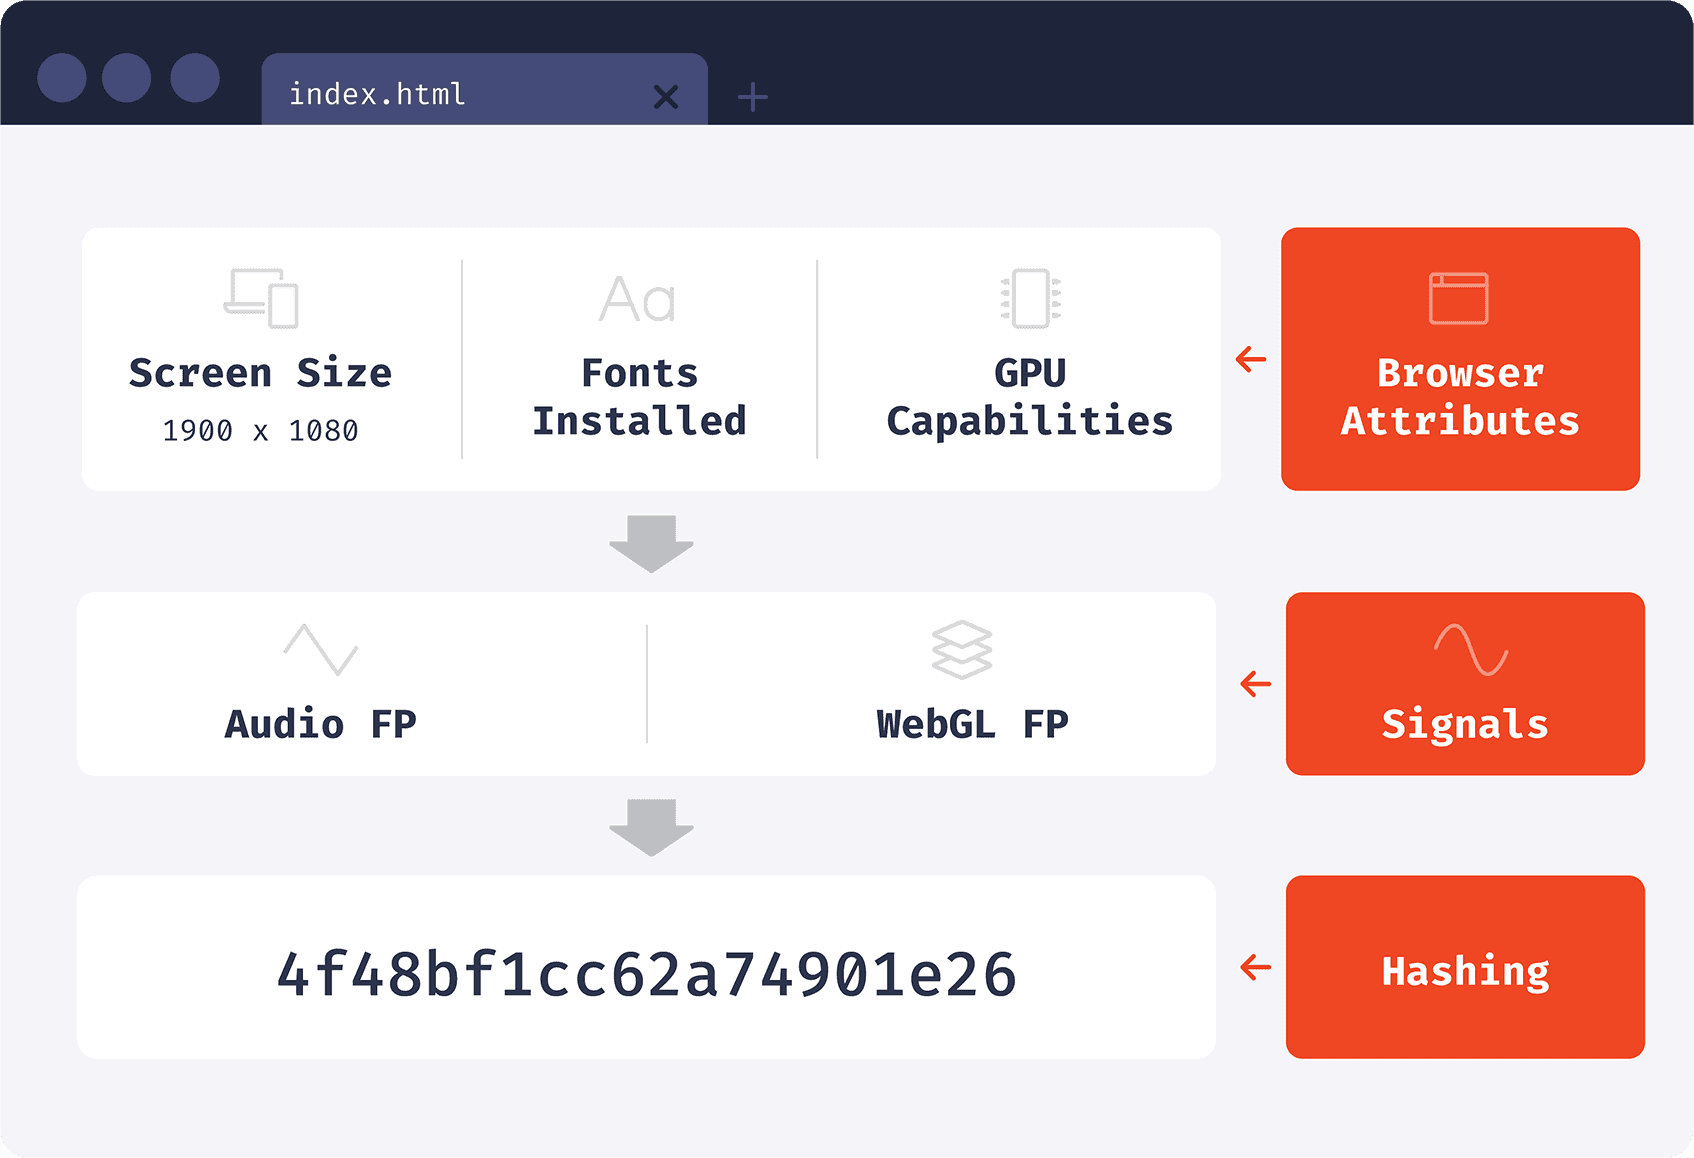
\includegraphics[width=.8\linewidth]{impl/browser_fingerprinting.png}
    \caption{Ausschnitt der genutzten Attribute zur Identifizierung des Browsers
    \cite{FingerprintJS2022}}
    \label{fig:impl-frontend-browser-fingerprinting}
\end{figure}

Nachdem die ID generiert wurde, wird sie als Nutzername und Passwort verwendet,
um einen neuen Account zu erstellen. Für alle weiteren Aktionen innerhalb der
Web-App, wie z. B. dem Besuchen von Stationen, wird der Account in der Anfrage
genutzt. Somit können die ausgeführten Aktionen im Nutzerprofil der
Teilnehmenden hinterlegt werden. Der Vorteil des Browser Fingerprinting liegt
hierbei in seiner Eigenschaft langlebig zu sein. Über mehrere Wochen kann
ein Browser Fingerprint für das gleiche Gerät unverändert bleiben. Somit ist die
Wahrscheinlichkeit hoch, dass selbst nach dem Löschen des Browserspeichers die
gleiche ID generiert wird. Folglich wird der gleiche Nutzeraccount verwendet und
ein Datenverlust vermieden.

\section{Implementierung des Dashboards} \label{sec:impl-dashboard}

In diesem Abschnitt wird die Implementierung des Dashboards präsentiert. Da es
sich hierbei um ein Strapi Plugin handelt, wird zunächst der Aufbau eines
Plugins beschrieben. Daraufhin wird die Implementierung der visuellen
Aufbereitung der Daten erläutert. Abschließend wird das Location-Picker Plugin
implementiert, welches die Eingabe von Standortdaten vereinfacht.

\subsection{Aufbau eines Strapi Plugins}

Nachdem in \ssecref{ssec:impl-backend-structure} bereits die grundlegende
Struktur eines Strapi Projekts erklärt wurde, wird in diesem Abschnitt der
Aufbau eines Plugins innerhalb Strapis näher erläutert.
%TODO: Continue

\subsection{Implementierung der Statistiken}

Eine der Hauptfunktionen des Dashboards ist das Überblicken der Veranstaltung
und seiner gesammelten Daten. Um dies zu ermöglichen wurden die Daten der
Teilnehmenden, Stationen und Abzeichen im Dashboard visuell aufbereitet.
Nachfolgend wird erklärt wie das \textit{victory-charts} Paket dazu genutzt
wurde, die Statistiken zu realisieren.
%TODO: Continue

\subsection{Implementierung des Location-Picker Plugins}

Der Standort einer Station ist eine seiner fundamentalen Informationen. Jedoch
besitzt Strapi keine vorhandene Oberfläche oder Datentyp um Standortdaten
einzutragen. Um die mühsame Eintragung von Longitude und Latitude zu vermeiden,
wurde ein Plugin implementiert, welches das Setzen eines Standorts mithilfe
einer interaktiven Karte ermöglicht. Im Folgenden wird die Implementierung
dieser mit erläutert.
%TODO: Continue

\section{Nutzung des Systems}

\subsection{Installation}

\subsection{Ausführung mit Docker}

\chapter{Evaluation} \label{chapter:evaluation}

Darauf folgend wurde das Framework im Rahmen der Stadt- und Campusrallye der
Vorwoche an der Universität zu Lübeck eingesetzt und anschließend evaluiert.
Hierzu wurde für Teilnehmende eine quantitative Online-Befragung durchgeführt,
während die Veranstaltenden im Anschluss zum Einsatz interviewt wurden.

\section{Teilnehmende}

\subsection{Methodik}

% Quantitative Befragung mit LimeSurvey

\subsection{Ergebnisse}

\section{Veranstaltende}

\subsection{Methodik}

\subsection{Ergebnisse}

\chapter{Zusammenfassung} \label{chapter:summary}

\section{Diskussion}

% Strapi Beschwerden
%   - Entwicker Erfahrung
%       - Schlechte Plugin Dokumentation
%       - Schlechte Helper-Plugin Dokumentation
%       - Tooling Probleme
%   - Rechtesystem
%       - Rechte der Gruppen nicht einstellbar
%       - Nur durch Aufpreis

\appendix

\setlength{\parskip}{2pt}

\chapter{Interviewleitfäden: Analyse} \label{appendix:interview}

\section{Teilnehmende}


\textbf{\large Einstieg}

\begin{enumerate}[noitemsep,topsep=0pt]
    \item Begrüßung und Danken für die Zeit
    \item Kurzer Umriss des Themas
    \item Ist die EMI-Award-App bekannt?
    \item Alter, Studiengang / Tätigkeit
    \item Kontaktmöglichkeit im Nachhinein
    \item Datenschutz
\end{enumerate}


\textbf{\large Einstiegsfrage}

\begin{enumerate}[noitemsep,topsep=0pt]
    \item {
        Welche von Ihnen besuchte Veranstaltung ist Ihr persönlicher Favorit?
        \begin{enumerate}[noitemsep,topsep=0pt]
            \item Berücksichtigen: Covid, lange keine Präsenz Veranstaltungen
            \item Details zur Veranstaltung erfragen, falls nicht bekannt
        \end{enumerate}
        }
    \item Was macht diese Veranstaltung zu ihrem persönlichen Favoriten?
\end{enumerate}


\textbf{\large Schlüsselfragen}

\textbf{Frage 1:} Wenn Sie sich etwas hilfreiches begleitend zur Veranstaltung wünschen könnten, was würde dies sein?

\textbf{Frage 2:} Welchen Technologien sind Sie auf Veranstaltungen schon begegnet? (Oder auch nicht)
\begin{itemize}[noitemsep,topsep=0pt]
    \item Hat Ihnen die Technologie auf der Veranstaltung geholfen?
    \item Wenn ja, wie? Sonst, warum nicht?
\end{itemize}

\textbf{Frage 3:} Wie wichtig ist Ihnen der soziale Austausch mit anderen Teilnehmenden während einer Veranstaltung?
\begin{itemize}[noitemsep,topsep=0pt]
    \item Wie verändert sich dies mit dem Typ der Veranstaltung?
\end{itemize}

\textbf{Frage 4:} Welchen (multi-/medialen) Weg bevorzugen Sie um Informationen aufzunehmen? (Videos schauen, Berichte/Artikel lesen, Podcasts hören, ...)
\begin{itemize}[noitemsep,topsep=0pt]
    \item Wie verändert sich dies in einem lehrreichen / unterhaltenden Setting?
\end{itemize}


\textbf{\large Abschluss}

\begin{enumerate}[noitemsep,topsep=0pt]
    \item Nochmals für die Zeit Danken
    \item Kontaktmöglichkeit im Nachhinein
    \item Verabschiedung
\end{enumerate}


\section{Veranstaltende}

\textbf{\large Einstieg}

\begin{enumerate}[noitemsep,topsep=0pt]
    \item Begrüßung und Danken für die Zeit
    \item Kurzer Umriss des Themas
    \item Vorerfahrung (Wie viele Veranstaltungen? Wie Groß?)
    \item Kontaktmöglichkeit im Nachhinein
    \item Datenschutz
\end{enumerate}

\textbf{\large Einstiegsfrage: Phase Organisation}

\begin{enumerate}[noitemsep,topsep=0pt]
    \item  Welche von Ihnen (mit)organisierte Veranstaltung ist Ihr persönlicher
          Favorit?
    \item {
          Beschreiben Sie grob den Ablauf bei der Planung der Veranstaltung
          \begin{enumerate}[noitemsep,topsep=0pt]
              \item Ob und wie wird Feedback von Teilnehmenden während Veranstaltung gesammelt?
              \item Ob und wie Kontakt zu Teilnehmenden während Veranstaltung?
              \item Ob und wie Kontakt zu Teilnehmenden nach Veranstaltung?
              \item Welche Priorität hat die Zugänglichkeit der Veranstaltung?
              \item Was wird für die Zugänglichkeit getan?
          \end{enumerate}
          }
\end{enumerate}


\textbf{\large Schlüsselfragen}

\textbf{Frage 1 (Organisation/Durchführung):} Wenn Sie sich etwas hilfreiches begleitend zur Veranstaltung wünschen könnten, was würde dies sein? Explizit Organisatorisch

\textbf{Frage 2 (Durchführung):} Was für Feedback ist während einer
Veranstaltung wichtig? (Worauf kann realistisch noch eingegangen werden?)
\begin{itemize}[noitemsep,topsep=0pt]
    \item Welche Daten werden benötigt in der Nachbereitung?
\end{itemize}

\textbf{Frage 3 (Durchführung/Nachbereitung):} Wenn die Möglichkeit bestände
Teilnehmer während einer Veranstaltung direkt / jeder Zeit anzusprechen, wofür
würden Sie das nutzen?
\begin{itemize}[noitemsep,topsep=0pt]
    \item Wofür nach einer Veranstaltung?
\end{itemize}

\textbf{\large Abschluss}

\begin{enumerate}[noitemsep,topsep=0pt]
    \item Nochmals für die Zeit Danken
    \item Kontaktmöglichkeit im Nachhinein
    \item Verabschiedung
\end{enumerate}

\chapter{Interviewleitfaden: Evaluation} \label{appendix:evaluation}

\textbf{\large Einstieg}

\begin{enumerate}[noitemsep,topsep=0pt]
    \item Begrüßung und Danken für die Zeit
    \item
        Gesamteindruck
        \begin{enumerate}[noitemsep,topsep=0pt]
            \item Was ist positiv aufgefallen?
            \item Was ist negativ aufgefallen?
        \end{enumerate}
        \begin{itemize}[noitemsep,topsep=0pt]
            \item[->] darauf dann wieder eingehen
        \end{itemize}
\end{enumerate}

\textbf{\large Details zum Ablauf }

\begin{enumerate}[noitemsep,topsep=0pt]
    \item  Wie lief das Erstellen der Veranstaltung?
    \begin{enumerate}[noitemsep,topsep=0pt]
        \item Eintragen der Informationen (Stationen, Abzeichen, Intro)
        \item Einstellen des Standorts
        \item optional aus Frage 2 übernehmen
    \end{enumerate}
    \item Wie lief das “Überwachen” der Veranstaltung?
    \begin{enumerate}[noitemsep,topsep=0pt]
              \item Einsehen der Statistiken
              \item Bewerten der Abzeichen
              \item Senden von Benachrichtigungen / Feedback
              \item Einstellen der Rahmendaten
              \item optional aus Frage 2 übernehmen
    \end{enumerate}
    \item Noch Ideen? Noch was gefehlt? Was vermisst du aktuell?
\end{enumerate}

\textbf{\large Abschluss}

\begin{enumerate}[noitemsep,topsep=0pt]
    \item Nochmals für die Zeit Danken
    \item Kontaktmöglichkeit im Nachhinein
    \item Verabschiedung
\end{enumerate}

\chapter{Digitale Medien}

Auf der beigefügten CD sind folgende Inhalte zu finden:
\begin{enumerate}[noitemsep,topsep=0pt]
    \item Aufnahmen der geführten Interviews (Verzeichnis \textit{/befragung})
    \item Detaillierte Ergebnisse der Evaluation (Verzeichnis \textit{/evaluation})
    \item Quellcode des entwickelten Systems (Verzeichnis \textit{/framework})
    \item PDF-Version dieser Arbeit
\end{enumerate}



\end{document}
